\documentclass[11pt, letterpaper]{book}
\usepackage{fontspec}
\usepackage{hyperref}
\usepackage{graphicx}

\usepackage{xgreek}    % greek hyphenation
\usepackage{titlepic}  % picture at title


\hypersetup{pdfborder=0 0 0, colorlinks=true, linkcolor=red}
\setmainfont[Ligatures=TeX]{Linux Libertine}

\newcommand\dialogue[1]{\par\noindent--~\textit{#1}}

\newcommand\photo[1]{\begin{center}\noindent\includegraphics[width=0.9\textwidth]{photos/#1}\end{center}}

\titlepic{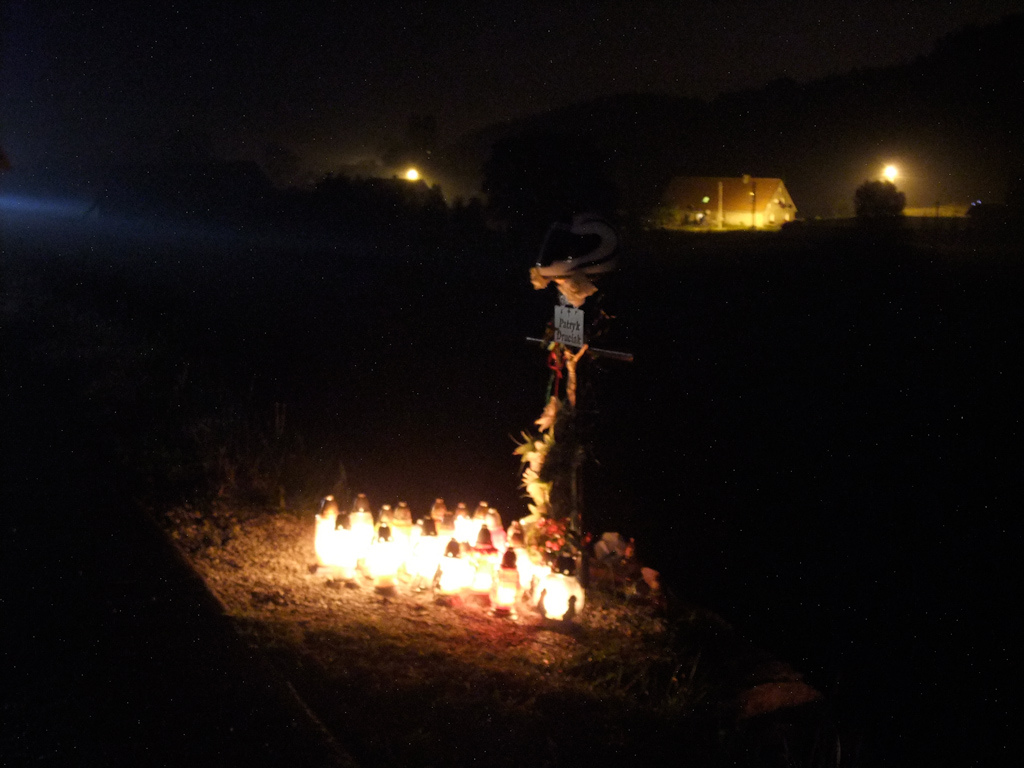
\includegraphics[width=\textwidth]{photos/front.jpg}}
\title{72ος Παράλληλος: Η μοναξιά του αναβάτη}
\author{Ταξιδευτής}

\begin{document}
\maketitle
\tableofcontents

\chapter{Εισαγωγή}

Αυτο το ταξιδι το χρωσταω σε ολους τους υπεροχους ανθρωπους που συναντησα καθ οδον, σε φιλους παροντες και εκεινους που δεν ειναι πια εδω... Christie, Κωστα, Γιαννη, Ion, Christian, Asa, Οle, Marko, Oili, Annika, Marek, Αlex, Dragan, Πετρο, Θαλεια, Κωστη, Μαθο, Πανο, Μανωλη, Γωγω... Χωρις εσας πολυ απλα δεν θα υπηρχε το ταξιδι τουτο και γι' αυτο και σας ανηκει.

Στο ραφι απεναντι μου, εκει, αναμεσα σε βιβλια παρτιτουρες και καθε λογης ματζαλα, εχω ενα σημειωματαριο με τους χαρτες απο το ταξιδι, γεματο με σημειωσεις για σκεψεις, εικονες, συναισθηματα. Ειναι καιρος τωρα που προσπαθω να το αποφυγω το ατιμο. Το εχω αφησει εκει και κανω οτι δεν το βλεπω ομως νοιωθω να με κοιταει απο απεναντι επικριτικα σαν να μου λεει ``Αντε! Ξεκινα! Γραψε!''

Ειναι αληθεια οτι καθε φορα που καθομαι να γραψω για ενα ταξιδι δυσκολευομαι. Αυτη τη φορα ομως ειναι διαφορετικα. Δεν ξερω....
Δεν ξερω αν μπορω να γραψω αρκετα καλα ωστε να μεταφερω το τι εζησα. Νοιωθω λιγος αυτη τη φορα γαμωτο!
Γραφω, σβηνω και ξαναγραφω, ξανασβηνω και τα παραταω. Γιατι ειναι τοσο δυσκολο να παρει η ευχη;

Αυτη η φωνη μεσα στο μυαλο δεν λεει να σωπασει.

\dialogue{Ξερεις το λογο Νικο.}
\dialogue{Σκασε.}
\dialogue{Ξερεις τι πρεπει να κανεις για να γραψεις.}
\dialogue{Ασε με!}
\dialogue{Για να γραψεις για αυτο το ταξιδι πρεπει να μπορεσεις να τα πεις ολα. Να παραδεχτεις αληθειες δυσκολες, να αντιμετωπισεις φαντασματα, να μηδενισεις κοντερ. Αντεχεις ρε φιλε; Εχεις τα αντερα να μην κρυφτεις απο τον ιδιο σου τον εαυτο; Εδω σε θελω....}

Ναι λοιπον ειναι καιρος να γραψω γιατι ολα αυτα μεσα δεν χωρουν πια...
Δεν γινεται να το αποφευγω πια... Στο ποτηρι εχει απο ωρα μπει ενα καλο single malt και απ' τα ηχεια η μοναδικη φωνη του Sivert Hoyem ερχεται να βαλει φωτια στα συναισθηματα, να πυρωσει μνημες και εικονες. Το soundtrack του ταξιδιου αυτου δεν θα μπορουσε να ξεκιναει αλλιως.... \href{http://goo.gl/xUsd7}{Sivert Hoyem - Give it a whirl}

\begin{verse}
\textit{It's my time to be waiting\\
Locked down, chained in the hole\\
But when my waiting is done I'm gonna give it a whirl...}\\
\end{verse}

Αυτο το ταξιδι ηταν οτι πιο δυσκολο εχω ζησει. Γιατι ομως; Ουτε ο πρωτος ουτε ο τελευταιος που πηγε στο Βορειο Ακρωτηρι ημουν.
Αλλοι πηγανε και περασαν ζαχαρη και ολα καλα και ωραια και χαλαρα και σουπερ γουαου.
Οχι εγω. Μπορει να ηταν Ονειρο ζωης, μια μοναδικη εμπειρια που θα κουβαλαω μεχρι να χτυπησω καρτα απο το ματαιο τουτο κοσμο, να ηταν κατι που χρωστουσα σε εμενα και σε αδερφια που δεν μπορεσαν να πανε ποτε, αλλα ευκολο ΔΕΝ ηταν...
Σωματικα, νοητικα, ψυχικα. Το ταξιδι αυτο ζητησε τα παντα και ακομα περισσοτερα. Καθε οριο, καθε κολλημα, καθε φοβια, καθε νοοτροπια. Οσο το αγαπησα τοσο το μισησα και οσο το θελησα αλλο τοσο το μετανοιωσα. Ψαχνετε να βρειτε λογικη; Διαβαστε κατι αλλο καλυτερα γιατι εδω δεν παιζει να τη βρειτε...

Αγκαλιασα το αγνωστο γιατι πολυ απλα δεν ειχα αλλες επιλογες και ειχα το χαμογελο του παλαβου καθως ο Μερφυ εκανε οτι μπορουσε για να μου χαλασει τη διαθεση.
Ειδα μερη αποκοσμα που δεν μπορουσα να φανταστω οτι υπαρχουν σε αυτο το πλανητη.
Εζησα καταστασεις τρελες και παλεψα με καθε ειδους συνθηκες. Απο τον καυσωνα των 42 βαθμων στο πολικο ψυχος του αρκτικου κυκλου, με ηλιο, με βροχη, αερα, χιονι και οτι αλλο μπορει να ριξει η φυση πανω σε ενα ταλαιπωρο μηχανοβιο ταξιδιωτη.
Ατελειωτα χιλιομετρα, στο ελεος και τις διαθεσεις του καιρου, κατω απο ενα βαρυ ουρανο, με συντροφο τη μηχανη μου... Εκει ειναι που κανεις φιλη τη μοναξια δικε μου γιατι αλλιως εισαι χαμενος απο χερι.

Ποσο ειρωνικο ομως ειναι οτι αναμετρηθηκα με οτι μπορουσα να φανταστω, για να ανακαλυψω οτι ο μεγαλυτερος εχθρος μου απο την αρχη ηταν ενας: Εγω.
Στο ταξιδι αυτο ομως τον εκανα μαγκα: τον γκρεμισα κομματι κομματι για να ανακαλυψω αυτο που κρυβοταν πισω απο τη σκουρια και τη μπιχλα της καθημερινοτητας και του βολεματος... Εγινα κατι αλλο απο αυτο που ημουν. Αυτο το ταξιδι σε αλλαζει βαθεια. Ειναι βασανιστικο, σκληρο αλλα τελικα λυτρωτικο...
Στο καθενα δινει την απαντηση σε οσα αναζητα. Σε εμενα εδωσε την απαντηση που γυρευα να βρω, και ας ηταν δυσκολη να την παραδεχτω...

Ταξιδευοντας εμαθα να εμπιστευομαι τους ανθρωπους που συνανταω, να ακολουθω το ενστικτο μου και πανω απο ολα να μη φοβαμαι κανεναν και τιποτα στο κοσμο. Παντα στα ταξιδια γυριζα λιγο διαφορετικος απο οτι εφευγα. 
Ομως αυτη τη φορα κατι αλλαξε οριστικα μεσα μου...
Μετα απο αυτο το ταξιδι.... δεν ξερω... νοιωθω να μπορω να κανω τα παντα και τιποτα πια...

Αν ψαχνετε ενα ταξιδιωτικο με λυρικες περιγραφες για τα φοβερα μερη που ειδαμε, για το ποσο τελεια ηταν ολα και το ποσο ωραια περασαμε, καλυτερα να σταματησετε να διαβαζετε εδω. Αν μη τι αλλο, υπαρχουν ενα σωρο αλλα ταξιδιωτικα εκει εξω απο παιδια που εχουν κανει αυτο το ταξιδι και τα μπορουν να τα πουνε πολυ καλυτερα απο εμενα ολα αυτα.

Αυτη εδω η ιστορια ειναι απλα οι σκεψεις ενος μονου αναβατη που προσπαθησε να κανει πραγματικοτητα ενα μεγαλο ονειρο -εικονες, συναισθηματα, νοηματα, ολα ατακτως ερριμενα.
Μη με παρεξηγησετε... Ισως βαζοντας τα στο χαρτι να βρω μια ακρη και να ξετυλιξω το κουβαρι...
Τι; Νομιζατε οτι θα τη γλυτωσετε ετσι απλα; Γελαστηκατε! Θα παρει χρονο το ταξιδιωτικο αυτο και δεν θα ειναι ευκολο.
Θα βγει με κοπο αλλα ισως και να αξιζε στο τελος -οπως εγινε και με το ιδιο το ταξιδι.

Σχολια, ευχες, παρατηρησεις, μπινελικια, ευχες και καταρες, ριψατε εντος. Ολα καλοδεχουμενα, σημαντικα, απολυτως απαραιτητα τελικα.

``There was nowhere to go but everywhere, so just keep on rolling under the stars.''

\photo{1.jpg}

\chapter{Day 0 -- Αθήνα (GR) - Ancona (IT)}

Το ταξιδι αυτο ηταν κατι που υπηρχε παντα μεσα στο μυαλο μου. Απο τοτε που θυμαμαι τον εαυτο μου σε δυο ροδες, παντα αναφερομουν στο ταξιδι στο Βορειο Ακρωτηρι σαν Το Ταξιδι. Eνα απο αυτα τα ονειρα που πρεπει να κανει καποιος πραγματικοτητα πριν κλεισει τα ματια.

Η φωτια σιγοκαιγε χρονια μεσα στο μυαλο αλλα καθε φορα που πηγαινε να φουντωσει την εσβηνα λεγοντας ``αστο μωρε, εχουμε χρονο, τωρα εξαλλου εχουμε το Χ, το Ψ, το Ω''. Καθε φορα μια δικαιολογια, καθε φορα μια αναβολη. Ωσπου ηρθε εκεινο το τηλεφωνημα εκεινη την ρημαδα Κυριακη του Σεπτεμβριου απο τον κολλητο.

\dialogue{Ελα ρε Νικο, που εισαι ρε και σε ψαχνω;}
\dialogue{Ελα φιλε, ειμαι σε κατι συγγενικες υποχρεωσεις. Τι εγινε;}
\dialogue{Δεν τα εμαθες; Ο Πανος ρε... Εφυγε...! Συνορα Ουκρανιας με ενα διερχομενο φορτηγο.}
\dialogue{........}

Ο καλος μου φιλος ο Πανος... Αδερφος ταξιδευτης και αυτος ειχε φαει τα Βαλκανια και την Ευρωπη με το κουταλι, και πλεον εγραφε ροτες για νοτια. Με εκεινον ειχα ξεκινησει το πρωτο μεγαλο μου ταξιδι στην Ευρωπη το 2007, με εκεινος ειχα κανει ενα σωρο βολτες και ταξιδακια οσο βρισκοταν Ελλαδα πριν μετακομισει Βουλγαρια. Μια μερα πριν μιλουσαμε γαμωτο! Και τωρα....

Εκει κατι αλλαξε μεσα μου. Ο χρονος που πριν ηταν απλετος τωρα ειχε τελειωσει. Οι δικαιολογιες, οι αναβολες εγιναν χιλια κομματια με τον πιο βιαιο τροπο. Τωρα. ΤΩΡΑ.
Μην αναβαλλεις δικε μου το Ονειρο γιατι μια μερα θα ειναι πολυ αργα. Παντα υπαρχει τροπος, αλλα ειναι πιο ευκολο να βρισκεις δικαιολογιες για να λες ``δεν μπορω''... Τα ονειρα ζητανε βλεπεις πολλα: θυσιες, κοπο και αιμα που βραζει. Πως να το κανεις οταν εισαι βολεμενος στο τακτοποιημενο, καθαρο, αποστειρωμενο κουτακι της ζωης σου; Το κουτι μου ομως εγω το ειχα σπασει και δεν κοιταζα πισω πια.

Γυρισα σπιτι αμιλητος, μουδιασμενος. Ανοιξα τους παλιους χαρτες γιατι ξερω οτι αυτο λατρευε και ξεκινησα να σχεδιαζω ροτες... Το ταξιδι ειχε ξεκινησει ηδη. Ενα ταξιδι που δεν προλαβε γαμωτο αλλα θα το καναμε μαζι.

Δυσκολοι μηνες περασαν απο τοτε, ομως το ονειρο δεν ξεχαστηκε. Δεν μιλησα σε κανεναν. Θα το εκανα μονο οταν ολα θα ηταν πλεον ετοιμα. Ηταν τοσα που θα μπορουσαν να πανε στραβα. Δουλεια, αδεια, χρονος, χρημα, διαθεση, μηχανη και αλλα τοσα απροβλεπτα και ξαφνικα.

Σιγα σιγα ξεκινησαν ετοιμασιες. Ο εξοπλισμος εκστρατειας ηταν απο πριν απολυτα ικανος να αντεξει ενα τετοιο ταξιδι, οποτε απλα αρχισα να μαζευω τα λιγα που μου ελειπαν: ενα καλο αδιαβροχο, ολοσωμο ισοθερμικο, νεα δερματινα, ενα κουζινακι για το μαγειρεμα... Λιγο πριν το καλοκαιρι η αδεια κανονιστηκε, οι διαδρομες αρχισαν να βγαινουν, το προγραμμα κανονιστηκε, τα πλοια εκλεισαν. Οταν ελαβα το πρωτο confirmation απο το πλοιο που θα με πηγαινε απο Δανια - Νορβηγια ενοιωσα μαγικα: το ονειρο επαιρνε πλεον σαρκα και οστα! Θα το εκανα!

Οι ημερομηνιες που επελεξα συγκεκριμενες: απο τα μεσα Ιουλιου μεχρι αρχες Αυγουστου. Ο λογος απλος: εκει πανω ο καιρος απο τον Αυγουστο και μετα αγριευει και θελει προσοχη. Η καλυτερη περιοδος για να επισκευτει καποιος αυτες τις χωρες ειναι απο τελη Ιουνιου μεχρι μεσα Αυγουστου. Χα! Ετσι ελεγαν.... Καθως οι μερες περνουσαν και εφτανε ο καιρος, το αγχος για το τι πηγαινα να κανω ολοενα και μεγαλωνε. Το να λες ``παω Βορειο Ακρωτηρι'' ειναι τρεις απλες λεξουλες, αλλα οταν το κανεις πραγματικα, εκει δικε μου ειναι ΕΝΤΕΛΩΣ αλλη ιστορια...

Η τελευταια βδομαδα πριν το ταξιδι περασε μεσα σε ενα πανικο δουλειας, πιεσης να τα προλαβω ολα και αγχους για να μην ξεχασω τιποτα.

Πεμπτη μεσημερι στο γραφειο και κατι περισσοτερο απο 24 ωρες για την αναχωρηση! Παρασκευη βραδυ θα επαιρνα το πλοιο απο Ηγουμενιτσα για Ανκονα. Ολα ηταν ετοιμα. Μεχρι που χτυπησε το τηλεφωνο:

\dialogue{Ναι γεια σας, τηλεφωνω απο την Greek Ferries. Eχετε κλεισει ενα εισιτηριο απο Ηγουμενιτσα για Ανκονα για αυριο το βραδυ;}
\dialogue{Ναι.}
\dialogue{Θελουμε να σας ενημερωσουμε οτι το πλοιο ακυρωνεται!}

Αφου συνηλθα απο το μινι εγκεφαλικο εγινε χαμος:

\dialogue{Μα τι μου λετε;;;;! Αυριο φευγω για 23 μερες ταξιδι και ολα ειναι κλεισμενα ηδη! Και μου λετε μια μερα πριν οτι ακυρωνεται το πλοιο;}
\dialogue{Ε ναι, μας ενημερωσαν απο την Superfast οτι το πλοιο αυτο πλεον δεν θα κανει αυτο το δρομολογιο. Μπορειτε να παρετε ενα αλλο πλοιο απο Ηγουμενιτσα στις 5 }το απογευμα.
\dialogue{Αυτο ΔΕΝ γινεται κυρια μου! Μεχρι το μεσημερι αυριο εργαζομαι και δεν μπορω να το φυγω νωριτερα. Αυτος ηταν και ο λογος που επελεξα το βραδυνο δρομολογιο.}
\dialogue{Τι να σας πω, υπαρχει και αλλο ενα που φευγει 12 το μεσημερι απο Πατρα.}
\dialogue{.....}

Εκλεισα γιατι αν μιλουσα με ενα ντουβαρι θα ειχα καλυτερη συνεννοηση και αρχισα πανικοβλητος να κοιταω εναλλακτικες. Πως θα προλαβαινα αυτα τα δρομολογια; Θα επρεπε να φυγω απο πρωι και να καταφερω να μην παω καν στο γραφειο -κατι παρα πολυ δυσκολο! Ακομα δεν ξεκινησαμε και αρχισε ο Μερφυ να κανει παιχνιδι; Τη βαψαμε!

Εκει ως απο (βαυαρικης) μηχανης θεος εμφανιστηκε ο αδερφος Κωστης. Του εξηγησα το προβλημα και ανελαβε δραση. Με τα κοννε του στις ακτοπλοικες της Πατρας εμαθε οτι το ιδιο το πλοιο που θα επαιρνα απο Ηγουμενιτσα το βραδυ εφευγε 5 το απογευμα απο την Πατρα! Απλα δεν εκανε σταση πλεον Ηγουμενιτσα αλλα πηγαινε Ανκονα απευθειας, κατι που η ηλιθια του πρακτορειου δεν γνωριζε καν!

Την καλω επι τοπου και τη βαζω να ψαξει με την Superfast. Αφου ενημερωνεται οτι οντως ετσι ειναι, κλεινουμε θεση στο νεο δρομολογιο και σημαινει ληξη συναγερμου! Επιστροφη στο σπιτι για ενα τελικο ελεγχο στα συστηματα της Αυρας: GPS, θερμαινομενα, MP3, ασφαλειες, φωτα...

Εχετε ακουσει για κανεναν που απλα εκανε μια αλλαγη λαδια και πηγε Βορειο Ακρωτηρι; Οχι; Ε τωρα θα ακουσετε! Το τελευταιο σερβις που της ειχα κανει ηταν στις 88.000 χλμ οποτε τωρα που ειχε αισιως μπει στις 100.000 το μονο που χρειαζοταν ουσιαστικα ηταν μια αλλαγη λαδιων που της χρωστουσα. Ολα τα αλλα ηταν μια χαρα! Τι αλλο να χρειαζοταν για το ταξιδι;

2 το πρωι, μεσα σε μια ζεστη, υγρη νυχτα του Ιουλιου, και οι βαλιτσες κουμπωναν πανω στην Αυρα.
Το μυαλο ακομα δεν μπορουσε να το χωρεσει αυτο που πηγαινα να κανω, αλλα τωρα δεν υπηρχε επιστροφη...
Η μερα της μεγαλης φυγης ξημερωνε συντομα.

\photo{2.jpg}

Το πρωι στο γραφειο τρελη πιεση να κλεισουν οι εκκρεμοτητες και πανικος να φυγω στην ωρα μου. 
Το αγχος του φευγιου. Πως θα γινει μια φορα να φυγω με το πασο μου; Τρεχουμε και δεν φτανουμε μια ζωη! 
Ο χρονος που νομιζεις οτι εχεις και τελικα ανακαλυπτεις οτι ποτε δεν ειναι αρκετος.

Ο Κωστης μου στελνει μηνυμα: ``Μην ξεχαστεις! Το πλοιο φευγει απο το νεο λιμανι στη Πατρα.'' Ιδεα δεν ειχα! Ποτε εφτιαξαν νεο λιμανι; Το 2010 ειχα φυγει απο το παλιο κλασσικο στην εισοδο της πολης. Το αλλαξαν;; 

Ευτυχως που με ενημερωσε γιατι ιδεα δεν ειχα! Μου δινει σχετικες οδηγιες και κανονιζουμε να συναντηθουμε στην εξοδο της περιφερειακης Πατρων για να με παει μεχρι το πλοιο. 

Κατεβαινω στη μηχανη σαν τον κυνηγημενο. Αγχος, στρες, πιεση, ουφ! Βαζω το κλειδι στη μιζα και... κοντοστεκομαι. Αυτο ειναι! Γυριζω μιζα και ξεκιναω να ζησω ενα ονειρο. Ενα κουμπι με χωριζει. Κλικ. Το μπασο γρυλισμα της Αυρας αντηχει στο υπογειο γκαραζ και εγω χαμογελαω σαν χαζος! Φυγαμε!

Η μηχανη κυλουσε σβελτα στην Εθνικη για Πατρα και το χαμογελο δεν ελεγε να φυγει απο τα χειλη μου. Η διαδρομη εκανε οτι μπορουσε να μου χαλασει τη διαθεση αλλα δεν εδινα σημασια. Μια βδομαδα τωρα οι θερμοκρασιες ηταν πανω απο 40 βαθμους και σε τετοιες συνθηκες το ταξιδι ειναι δραματικο. Η ζεστη χτυπουσε κοκκινα και ο αερας ηταν τοσο καυτος που εκλεισα ζελατινα για να δροσιστω.  Η υπνηλια απο την ανυποφορη ζεστη και τη βαρεμαρα καραδοκουσε και τα χιλιομετρα παντα φαινονται περισσοτερα σε τετοιες συνθηκες..

Μετα απο εναν αιωνα περνουσα πλεον εξω απο τη Πατρα. Η ωρα ηδη περασμενες 4! Ειχα κατι λιγοτερο απο μια ωρα για το πλοιο.  Στη περιφερειακη Πατρων το αγχος για το αν προσπερασα τη σωστη εξοδο η οχι αρχισε να ερχεται ξανα. Ημουν οριακα σε χρονο. Αν επρεπε να γυρισω πισω και να ψαχνω το πλοιο το ειχα χασει!

Πανω που αρχισα να σκεφτομαι οτι ισως να ειχα κανει βλακεια ηρθε η θεα της σωστης πινακιδας να με ανακουφισει!

Ο Κωστης με το Φωτη με περιμεναν απο ωρα στη γεφυρα. Χαμογελο. Υπεροχο συναισθημα κ τοσο τιμητικο να σε μετρανε τοσο οι φιλοι που να καθονται να περιμενουν κατω απο το λιοπυρι για παρτη σου! 

Φυγαμε για το λιμανι συνοδεια. Ο Κωστης με την Μπεμπα μπροστα, ο Φωτης με το αγριμι πισω και η Αυρα φορτωμενη στη μεση. Μα ποιος ειμαι επιτελους; 

Το λιμανη ηταν χωμενο κυριολεκτικα στου διαολου το κερατο. Εγω απο μονος μου δεν θα το εβρισκα εγκαιρως με τιποτα. Ο Κωστης εσωσε το ταξιδι, κυριολεκτικα. Τυπικοτητες στο τσεκ ιν και φυγαμε για το πλοιο που ηταν ετοιμο για αναχωρηση.

Η ωρα ειχε περασει. Ο Κωστης γυρισε στο μερος μου και μου ειπε σε τονο υπηρεσιακο ``Φυγε, απο εδω και μετα ειναι ελεγχομενος χωρος. Ζησε το ονειρο σε καθε στιγμη και καλη ανταμωση.'' Ο χρονος ετρεχε και επρεπε να φυγω ομως ξερω τον Κωστη: λακωνικος, ομως δυο κουβεντες του ισοδυναμουν με χιλιες συζητησεις. Αντιο παιδια και θα τα ξαναπουμε.

\photo{3.jpg}

Δεσαμε τη μηχανη στο αμπαρι, διπλα σε ενα Ducati. Που ηταν ολοι οι αλλοι ταξιδιωτες; Ανεβηκα επανω και εκανα την καθιερωμενη βολτα στους οροφους του πλοιου...  Ομορφο, καινουργιο και καθαρο, ομως δεν εβρισκα μερος που να μπορει να ξαπλωσει κανεις. Που ειναι οι καναπεδες ρε παιδια; Βγηκα στο καταστρωμα ενω το πλοιο ειχε πιασει να σαλπαρει. Βλεπω την ακτη να χανεται κ μαζι της νοιωθω να χανονται και οι σκεψεις, το αγχος, τα προβληματα.. Το μονο που εχει σημασια πλεον ειναι το ταξιδι. Καθε μερα και αλλου, αλητεια κ περιπλανηση, αγνωστα μερη και περιπετεια. Να μην ξερεις τι σε ξημερωνει και να εχεις για μπουσουλα τον οριζοντα.

\photo{4.jpg}

Tο πλοιο ηταν σχεδον αδειο παροτι ημασταν στη μεση του καλοκαιριου. Προφανως λιγοι ειναι οι τρελοι που θελουν (και μπορουν πλεον!) καταμεσης του καλοκαιριου να φυγουν απο Ελλαδα. Φανταζομοαι οτι στην επιστροφη για Πατρα οι τουριστες θα κρεμονταν απο τα ρελια σαν τσαμπια! Ετσι ομως τωρα ηταν καπως καταθλιπτικο το θεαμα -μονο ενα τσουρμο πιτσιρικια γερμανακια φτιαχνουν λιγο την ατμοσφαιρα και μου θυμιζουν οτι ο κοσμος φευγει σε διακοπες.

Ο Νορβηγος φιλος Ole μου εστειλε μηνυμα, φτιαχοντας μου τη διαθεση: ο καιρος εκει πολλα υποσχομενος: ηλιος και 21 βαθμοι σημερα, το μεγαλυτερο που ειχαν δει λεει μεχρι τωρα! Τωρα τι του λες;

Η νυχτα επεσε σιγα σιγα και εγω αρχισα να ψαχνω ενα μερος να την πεσω. Μπρος γκρεμος και πισω ρεμα. Στο σαλονι, τηρωντας τις ενδοξες θαλασσινες παραδοσεις, το αircondition δουλευε τερμα γκαζια: οι θερμοκρασιες μπορει να χαροποιουσαν εναν πιγκουινο αλλα οχι εμενα. Απο την αλλη το καταστρωμα ηταν ζεστο αλλα τα πλαστικα παγκακια δεν τα ελεγες ακριβως και ιδανικα για υπνο. Λαγοκοιμαμαι δυο ωρες με τα φωτα φθοριου στα ματια και σηκωνομαι. Επιστροφη στο σαλονι οπου βρισκω μια καπως ευρυχωρη καρεκλα και κοιμαμαι σαν τελικο σιγμα. Superfast και υπνος ...ελευθερας βοσκης δεν πανε μαζι. 

Το πρωινο ξημερωσε με εναν λαμπρο ηλιο να ανατελλει πανω απο τη θαλασσα. Μοναδικο θεαμα να σε ξυπναει κατι τετοιο...

Σηκωθηκα και βγηκα στο καταστρωμα. Πηρα τον κλασσικο βαπορισιο καφε και αραξα σε μια μερια να απολαυσω τη στιγμη. Στο MP3 οι \href{http://goo.gl/HcaG4}{Starsailor} και οι \href{http://goo.gl/6sdDG}{Oasis} (κλικ ντεεεε!) εφτιαχναν το ιδανικο soundtrack της μερας:

\begin{verse}
There's a fever
On the freeway
In the morning

And the lover
Smiling for me
Without warning

There's an outlaw
On the highway
And she's falling

Man I must have been blind
To carry a torch
For most of my life

These days I'm hanging around
You're out of my heart
And out of my town...
\end{verse}

Αραχτος στο καταστρωμα, με το Zen and the art of Motorcycle Maintenance ανα χειρας, υπεροχος ηλιος, ζεστη, καφεδακι, μουσικη και κατω στο γκαραζ η Αυρα πανετοιμη να περιμενει να φυγουμε! Η Τελεια Στιγμη...

Σε λιγο το πλοιο πιανει λιμανι στην Ancona. Τι μας περιμενει καλη μου;

\photo{5.jpg}

\chapter{Day 1 -- Ancona (IT) - Como (IT) -- 492km}

Η ωρα πανω στα πλοια περναει αργα. Οσοι εχουν ταξιδεψει ετσι ξερουν. Κοιταξα το ρολοι μου. Με τη διαφορα ωρας θα επρεπε να κοντευουμε στο λιμανι. Ομως τριγυρω το μονο που βλεπω ειναι το απειρο μπλε της θαλασσας. Τι ωρα φτανουμε; Η απαντηση απο τον λογιστη του πλοιου με ξαφνιασε: 1 το μεσημερι;! Εγω πως νομιζα οτι φτανουμε 10.30 το πρωι; Η ιδεα μου να χαζεψω στους επαρχιακους δρομους της κεντρικης Ιταλιας τωρα πηγαινε απατη...

Η ωρα τελικα περασε χαζευοντας τους χαρτες για να δω τις διαδρομες που θα ακολουθησω για το προορισμο μου. Τι πιο ομορφο πραγμα απο αυτο; Να ξεκινας τη μερα σου χαζευοντας ολες αυτες τις μικρες πολυχρωμες γραμμουλες πανω στους χαρτες και να προγραμματιζεις αγνωστες διαδρομες για να νυχτωθεις οπου σε βγαλει ο δρομος...

Εγω ομως σημερα ειχα προορισμο: τη λιμνη Como, τη τριτη μεγαλυτερη λιμνη της Ιταλιας στα βορειοδυτικα της χωρας, ακριβως πανω στα Ιταλο-ελβετικα συνορα. Εκει ειναι και το ομωνυμο φημισμενο χωριο που αποτελει ενα (αρκετα κυριλε/ακριβο) τουριστικο θερετρο για τους Ευρωπαιους και οχι μονο, καθως ειναι και το μερος που ζει ο ...George εδω και χρονια. (Μη με ρωτησετε ποιος ειναι ο George ετσι; )
Ηθελα να επισκευτω την περιοχη εδω και χρονια και να που ειχε ερθει η ευκαιρια να το κανω. Βεβαια με το πλοιο να δενει τοσο αργα στην Ancona και εχοντας να διασχισω ουσιαστικα ολη την Ιταλια δεν θα εβλεπα και πολλα απο το Como αλλα δεν πειραζει. Ακομα και ετσι θα επαιρνα μια μικρη γευση!

\photo{6.jpg}

Το πλοιο ειχε πιασει να μπαινει στο λιμανι της Ancona και βρηκα την ευκαιρια να χαζεψω τριγυρω...
Δεν θα το ελεγα ακριβως ωραιο το μερος -ενα μικρο, μαλλον αδιαφορο λιμανακι ηταν αλλα ακομα και ετσι μερικα κτηρια διατηρουσαν την περιφημη Ιταλικη φινετσα και ομορφια...

\photo{7.jpg}

Κατεβηκα στο γκαραζ για να ετοιμαστω. Οσοι με ξερουν γνωριζουν οτι με το χρονο εχω μια πολυ περιεργη σχεση: μια ζωη αργω σε οτι και να κανω -και αυτη η φορα ΔΕΝ ηταν η εξαιρεση.

Τα παιδια με το Multistrada που ηταν παρκαρισμενο διπλα μου ειχαν ηδη κατεβει κατω και περιμεναν υπομονετικα να μαζεψω το τσαντιρι για να φυγουν. Οι παρκαδοροι του πλοιου θελοντας να διευκολυνουν την κατασταση επιασαν να λυνουν τους ιμαντες απο τις μηχανες για να φυγουμε μια ωρα αρχιτερα -ποσο μα ποσο θα το μετανοιωνα αυτο πολυ συντομα....

Για να βοηθησω με τη σειρα μου το ζευγαρι να φυγει μετακινησα την Αυρα 2 μετρα πιο πισω. Ομως εκει που την πηγα το πατωμα ειχε ενα μικρο εξογκωμα. 
Οχι και τοσο σημαντικο θα μου πειτε. Θα συμφωνουσα αν δεν υπηρχαν δυο μικρες λεπτομερειες:

1. Η μηχανη λογω βαρους απο τις βαλιτσες (και λογω εγκεφαλικης βλακειας δικης μου που ΔΕΝ εσφιξα την προφορτιση πριν το ταξιδι) εκανε την αναρτηση να βυθιζεται ελαφρα, ετσι ωστε οταν καθοταν στο stand πλαγιαζε απο λιγο εως ελαχιστα.
2. Οι ιμαντες δεσιματος ειχαν λυθει εντελως.

Ετσι εβαλα το stand αφου ειχα κανει πισω να φυγουν τα παιδια και πηγα πισω στη βαλιτσα να κλεισω απλα το καπακι. Καπου εκει εκανα την ενδιαφερουσα παρατηρηση οτι η μηχανη στηριζοταν σε οριακα ορθια θεση και καθως ακουμπαω το καπακι της βαλιτσας.... ο Τιτανικος βυθιζεται!
340+ κιλα πλαστικων και μεταλλων εφυγαν προς τα δεξια με χαρη που θα ζηλευε και ο ελεφαντας του Circo Medrano. Προφανως οι προσπαθειες να σταματησω το θηριο τραβωντας απο αριστερα ηταν εντελως αναξιες λογου και ετσι βρεθηκα να κοιταω τη μηχανη φαρδια πλατια στο καταστρωμα του πλοιου!

Τι πιο ωραια αρχη για το μεγαλυτερο ταξιδι που θα εκανα ποτε; 
Τελικα αν δεν πεσει η μηχανη μια φορα σε ενα ταξιδι μου δεν θα παει καλα. Το 2010 ειχε συμβει το ιδιο ακριβως 2 φορες αλλα το ταξιδι ειχε παει υπεροχα. Απο την αλλη να πω τωρα οτι χαιρομουν θα ημουν ψευτης...

Σηκωσαμε τη μηχανη πανω μαζι με ενα νταλικιερη που προθυμοποιηθηκε και ...ευτυχως σχεδον καμια ζημια! Η μηχανη ειχε κατσει πανω στη δεξια βαλιτσα σωζοντας τα χειροτερα και το μονο αλλο που ειχε βρει ηταν ενα πολυ μικρο πλαστικο στο δεξι φλας που γεμισε γρατζουνιες. Παλι καλα!

Αυτο που ειχε παθει ομως καλη ζημια ηταν το μεγαλο δαχτυλο μου στο δεξι χερι που πρηστηκε σχεδον αμεσως και δεν μπορουσε να κλεισει. Κακωση; Καταγμα; Το σιγουρο ηταν οτι ποναγε διαολεμενα. Πως θα ταξιδευα ετσι 12.000 χιλιομετρα; Αν ηξερα ομως τι θα ακολουθουσε μεχρι να τελειωσει αυτη η απιστευτη περιπετεια μαλλον θα το προσπερνουσα αυτο ως κατι αναξιο λογου βρε αδερφε...

Καθως ομως η Αυρα ρολαριζε τις ροδες της για μια ακομα φορα επι Ιταλικου εδαφους τα ειχα ξεχασει ολα και χαμογελουσα σαν χαζος...

\photo{8.jpg}

Σταματησα στο πρωτο βενζιναδικο που βρηκα για να ταισω τα αλογα και να αποφασισω για τη διαδρομη. Ηθελα πολυ να βγω στους επαρχιακους δρομους αλλα το GPS μου εκοψε τα ποδια: 10+ ωρες συνεχους οδηγησης και η ωρα ηταν ηδη 2 το μεσημερι. Στην καλυτερη των περιπτωσεων και χωρις καμια σταση (κατι πρακτικα αδυνατον) θα εφτανα τις 12 το βραδυ και βεβαια χωρις να εχω κανονισει καπου να μεινω δεν ηταν και η καλυτερη ιδεα να ψαχνω μεσα στη μαυρη νυχτα καπου να κοιμηθω...

Συνεπως autostrada και ξερο ψωμι για σημερα δυστυχως.
Και το δυστυχως οχι γιατι ειναι κανενας παλιοδρομος (αν και δεν μπορει φυσικα να συγκριθει με το ΥΠΕΡΤΑΤΟ μεγαλειο της Κορινθου - Πατρων) αλλα γιατι εγω βαριεμαι τρομερα τις εθνικες οδους και τις ευθειες και τις αποφευγω οπως ο Lemmy τη Britney Spears. Αναγκαιο ομως κακο σημερα η εθνικη αν ηθελα να φτασω σε καποια λογικη ωρα στο προορισμο μου.

Περα απο τη πλακα βεβαια η autostrada ειναι δρομαρα και αυτο δεν κρυβοταν με τιποτα...

\photo{9.jpg}

...ενω και οι εικονες της επαρχιακης ζωης τριγυρω εκαναν οτι μπορουσαν για να μην πληττω.

\photo{10.jpg}

Συντομα επιασα ρυθμο και η μηχανη αρχισε να τρωει τα χιλιομετρα γουργουριζοντας χαρουμενη, κατι που δεν μπορουσα να πω και για εμενα. Τρελη ζεστη, ηλιος και δερματινα δεν ειναι και ο καλυτερος συνδιασμος. 
Οι στασεις για νερο ηταν συνεχεις και παροτι ανεβαινα ολοενα και πιο βορεια η καψα του μεσογειακου καλοκαιριου δεν ελεγε να κοπασει παρα τα συννεφα που εβλεπα να μαζευονται πλεον στον οριζοντα. 
Τωρα ειχε και ζεστη και μουνταδα!

\photo{11.jpg}

Βγηκα απο την autostrada και προετοιμαστηκα για τις πραξεις ΧΧΧ που θα μου εκαναν στα διοδια: 27 ευρω για 400+ χιλιομετρα; Χμμμ! Περιμενα χειροτερα.
Το απογευμα ειχε πιασει να πεφτει απο ωρα και ανηφοριζα πλεον προς το Como. Ειχε βρεξει εδω πριν λιγο... Ο ουρανος γκριζος πλεον με βαρια συννεφα -θα προτιμουσα λιακαδα, αλλα οι μυρωδιες της φυσης και η ατμοσφαιρικη εικονα που εφτιαχνε ο ουρανος ηταν εξισου ομορφες...

Καθως κατεβαινα απο την εξοδο του δρομου προς τη λιμνη, το Como αρχισε να αποκαλυπτει το λογο γιατι θεωρειται ενας απο τους πιο ομορφους καλοκαιρινους προορισμους στην Ευρωπη.
Εκανα μια σταση στην ακρη του δρομου και τα ματια δεν μπορουσαν να χορτασουν τις εικονες...
Εικονες μιας ταινιας προσεχως...

\photo{12.jpg}
\photo{13.jpg}

To τοπιο ηταν απλα μαγευτικο! Με καποιο παραξενο τροπο η μουνταδα του ουρανου ταιριαζε απολυτα στη στιγμη εκεινη και εγω καθισα σιωπηλος χαμενος στη στιγμη...

\photo{14.jpg}

Θα ηθελα να κανω το γυρο της λιμνης αλλα η ωρα δεν το επετρεπε. Η νυχτα επεφτε πλεον και εγω ακομα δεν ειχα βρει που θα εμενα το βραδυ. Παρολαυτα, η διαδρομη που ξεκινουσε γυρω απο το Como εδειχνε πολλα υποσχομενη και στο μυαλο μου ανανεωσα το ραντεβου μου με την περιοχη για καποια αλλη φορα στο μελλον. Τελικα αν κατσω και βαλω ενα σημαιακι στα μερη που εχω αφησει στα ``προσεχως'' στο τελος δεν θα βλεπω χαρτη για χαρτη!

\photo{15.jpg}
\photo{16.jpg}

Το GPS εδωσε τη λυση για καποιο κοντινο camping: Camping Europa, ενα συμπαθητικο καμπινγκ ακριβως στην εξοδο του χωριου.

\photo{17.jpg}

Δυστυχως ομως η ρεσεψιον οσον αφορουσε την εξυπηρετηση και τη συννενοηση βρισκοταν στο απολυτο μηδεν: ενας βαριεστημενος πιτσιρικας (που ειμαι σιγουρος οτι θα προτιμουσε να ειναι οπουδηποτε αλλου εκεινη την ωρα) μετα βιας εδειχνε ενδιαφερον να εξυπηρετησει ενα ταλαιπωρημενο μηχανοβιο που στεκοταν μπροστα του.
Με τα ελαχιστα ιταλικα μου ευτυχως συνεννοηθηκαμε και μετα τις τυπικες διαδικασιες ξεκινησα να στησω τα συμπραγκ... Επ! Οχι τοσο γρηγορα φιλε μου! Ο καιρος δεν ειχε πει την τελευταια του λεξη ακομα...
Ισα που ειχα προλαβει να απλωσω το εσωτερικο της σκηνης, οταν αρχισαν να πεφτουν δυνατοι κεραυνοι πανω απο τη λιμνη και η ατμοσφαιρα γεμισε τη γνωριμη μυρωδια του οζοντος -σημαδι οτι εντος δευτερολεπτων θα ξεκινουσε ο κατακλυσμος του Νωε!
Τα πυκνα φυλλωματα των δεντρων απο πανω μου θα κρατουσαν μια μικρη βροχουλα αλλα κατι μου ελεγε οτι αυτο που ερχοταν μονο μικρο δεν θα το ελεγες... 

Μαζεψα αρον αρον τη σκηνη και ετρεξα πισω στη ρεσεψιον ενω η βροχη αρχισε να δυναμωνει. 
Καλυβακι; Λαστ γιαρ! Και τωρα τι κανουμε; Να στησω υπο βροχη ηταν κατι που θα προτιμουσα να αποφυγω...
Εν μεσω βροχης το πιτσιρικι μου προτεινε ενα τροχοσπιτο. Πως ειπατε; 
Το καμπινγκ ειχε μερικα παναρχαια, ταλαιπωρημενα τροχοσπιτα στημενα εκει μονιμα ως λυση αναγκης για οσους ηθελαν καλυβακι αλλα δεν εβρισκαν.

Μου εδωσε ενα κλειδι και μου ειπε το νουμερο που επρεπε να βρω. Που ειναι ρε παιδια το νουμερο 12; Δεν υπηρχε πουθενα! Μετα απο τρια τεσσερα πανω κατω στη ρεσεψιον φορωντας τα δερματινα και ιδρωνοντας σαν γουρουνι στο σακι ΠΑΡΑ τη βροχη που επεφτε τελικα καταφερα να εντοπισω το περιφημο τροχοσπιτο. 

Κατι που τελικα μακαρι να μην το ειχα κανει και ποτε! Ολη μου τη ζωη την εχω περασει σε καμπινγκ -ε λοιπον δεν εχω δει ΠΟΤΕ αλλοτε ενα τροχοσπιτο σε τοσο αθλια κατασταση. Τα παντα ηταν σκουριασμενα και σπασμενα. Πομολα, μεντεσεδες στις πορτες, μπρατσα στηριξης στα παραθυρα... Το μεγαλυτερο μερος του τροχοσπιτου εκτελουσε χρεη (σκουπιδ)αποθηκης με οτι σαβουρα μπορει να φανταστει κανεις πεταμενη μεσα ενω το κρεβατι ειχε επανω κατι τεραστιους λεκεδες που θα προτιμουσα να μην ξερω απο τι εγιναν και μια εκλεκτη κολεξιον απο ``Πεθαμενα ζωυφια αγνωστου ταυτοτητας'' του 2012. 
Σαν να μην εφταναν αυτα, το τροχοσπιτο εδειχνε να ...κατοικειται ηδη! Στο τοιχο υπηρχαν κατι ρωσικα εικονισματα και σε μια καρεκλα κατι παλια ρουχα και παντοφλες καποιου αντρα.

Μεσα σε χρονο μηδεν ημουν και παλι στη ρεσεψιον: αστο φιλε, θα το ρισκαρω με τη καταιγιδα χιλιες φορες παρα αυτο το πραγμα!
Εξαλλου με ολα αυτα η μπορα ειχε σταματησει πλεον οποτε χιλιες φορες η σκηνη μου και η φυση παρα να κλειστω σε ενα αθλιο κουτι.

Αραξα τη μηχανη σε ενα ωραιο σημειο που δεν ειχε βραχει πολυ και αρχισα να στηνω. 
Λιγα μετρα πιο περα δυο αλλες ταξιδιαρες μηχανες ηταν αραγμενες: ενα RT1100 και ενα GS1150, που αν εκρινα απο τα αυτοκολλητα και τη κατασταση τους μαλλον ειχαν να πουν πολλες ιστοριες για ταξιδια. 
Βρετανικες πινακιδες με Ουαλλικα διακριτικα! Συντοπιτες.

Καθως το βραδυ ειχε πεσει πλεον το τσαρδι ηταν ετοιμο και ειχα ηδη πιασει να μαγειρεψω κατι για δειπνο...
Καπου εκει ηρθαν και οι Ουαλλοι και κατσαμε να τα πουμε υπο τη συνοδεια παγωμενης μπυριτσας. 
Πολυ ωραιοι τυποι! Παλιοσειρες μηχανοβιοι ταξιδιωτες που ειχαν φαει την Ευρωπη με το κουταλι. Ειχαν ξεκινησει απο Αγγλια πριν μια βδομαδα και αυριο θα ξεκινουσαν να δουν τα πασα της Ελβετιας οπως και εγω! Οι ιστοριες και οι διαδρομες στους χαρτες εδιναν και επαιρναν μεχρι αργα το βραδυ...

Κρατηστε τα πιο κυριλε εστιατορια και τα πιο γκουρμε φαγητα σας. Εγω ετσι τωρα ημουν ο πιο ευτυχισμενος ανθρωπος του κοσμου. Μια σκηνη, η μηχανη διπλα, οι μποτες μου, αναπαντεχες συναντησεις και ενα ζεστο πιατο φαι στο τελος της μερας. Παραδεισος! 
Αυριο ξημερωνε μια νεα μερα...

\photo{18.jpg}

\chapter{Day 2 -- Como (IT) - Guebwiller (FR) 430 km}

Το ξημερωμα με βρηκε πτωμα. Ο αθλιος υπνος που ειχα κανει μεσα στο Superfast και τα 500+ χιλιομετρα μεσα στον πρωτοφανη για την Ιταλια καυσωνα ειχαν κανει αισθητη την επιδραση τους σε ενα σωμα που ειχε μεχρι προτινος καλομαθει σε ολες τις καθημερινες ανεσεις. Η ωρα ηταν περασμενες 8 και παροτι ηθελα να συνεχισω να κοιμαμαι ηξερα οτι επρεπε να σηκωθω αν ηθελα να βγαλω το προγραμμα της ημερας οπως ειχα σχεδιασει. Εξαλλου η πρωινη ζωη του camping που ειχε ξεκινησει εδω και ωρα δεν θα με αφηνε να κοιμαμαι για πολυ ακομα και να ηθελα...

\photo{19.jpg}

Ο προορισμος μου για σημερα ηταν η Γαλλια και συγκεκριμενα το Guebwiller στη νοτιοανατολικη Αλσατια οπου θα συναντουσα τη Christie: ενα μελος του Couchsurfing που μου ειχε προσφερει με χαρα να με φιλοξενησει στο σπιτι της αφου θα περνουσα απο την περιοχη. Γιατι ομως εκει; Διοτι σε αποσταση λιγων χιλιομετρων ηταν το περιφημο \href{http://en.wikipedia.org/wiki/Colmar}{Colmar}: καποιοι το ανεφεραν ως τη πιο ομορφη πολη της Ευρωπης και δεν θα αφηνα να παει χαμενη η ευκαιρια να διαπιστωσω αν ηταν αυτο ηταν αληθεια...

Πριν απο αυτο ομως σημερα θα επαιρνα την εκδικηση μου για τα βαρετα χιλιομετρα εθνικης που ειχα γραψει χθες! Ειχα να διασχισω την Ελβετια και σκοπευα να κινηθω οσο μπορουσα σε επαρχιακους δρομους και να απολαυσω τη μεγαλειωση φυση της χωρας αλλα βεβαια το μεγαλυτερο κερασακι ηταν αλλο: τα διασημα πασα Furkapass και Grimselpass στα 2.400 μετρα υψομετρο στην ραχη των Ελβετικων Αλπεων.
Οταν εχεις ενα τετοιο προγραμμα ξυπνας πιο ευχαριστα οσο να ναι...

\photo{20.jpg}

Πρωτα απο ολα ομως καφες. Οι Ουαλλοι διπλα ειχαν σηκωθει απο ωρα και επιναν ηδη το τσαι τους χαμογελαστοι, ενω δεν εχασαν ευκαιρια να μου την πουν οτι παρακοιμηθηκα κιολας! Οι παλιολυκοι μου εβαλαν τα γυαλια!
Ζεστανα νερο στο κουζινακι και εφτιαξα τον καφε μου και εκατσα να τον απολαυσω πλαι στους χαρτες μου και με παρεα αλλους μηχανοβιους ταξιδιωτες.
Το εχω πει πολλες φορες και θα το πω αλλες τοσες: δεν υπαρχει καλυτερος τροπος απο το να ξεκινας ετσι τη μερα σου!

\photo{21.jpg}

Οι Ουαλλοι μου ελεγαν οτι θα ακολουθησουν πανω κατω την ιδια διαδρομη με εμενα, τουλαχιστον μεχρι τα πρωτα πασα. Εκανα τη σκεψη να παμε μεχρι εκει παρεα ομως τους ειδα να βιαζονται να ξεκινησουν: εγω δεν ειχα προλαβει να πιω ακομα τον καφε μου και αυτοι ειχαν ξεστησει τις σκηνες τους και ειχαν σχεδον πακεταρει τα παντα! 
Αρχισα να μαζευω τα πραγματα βιαστικα αλλα καταλαβα οτι απλα θα τους καθυστερουσα χωρις λογο και εγω θα αγχωνομουν αδικα. Ανταλλαξαμε συμβουλες για τη διαδρομη και χαιρετηθηκαμε -μπορει να τα λεγαμε και στη πορεια εξαλλου!

Το πακεταρισμα παντα ηταν για εμενα ενα θεμα: μου τρωει χρονο. Πολυ χρονο. Μεχρι να μαζεψω υπνοσακους, υποστρωματα, σκηνη, τεντες, ρουχα και λοιπα συμπραγκαλα οι περισσοτεροι γειτονες ειχαν φυγει ηδη! Οκ, βεβαια πολλοι ηταν με τροχοσπιτα και αυτοκινητα αλλα οπως και να το κανεις ειναι αποκαρδιωτικο να παλευεις να σφηνωσεις ολα τα μπαγκαζια στις βαλιτσες και να βλεπεις τους αλλους να ξεστηνουν τα παντα χαμογελαστοι στο χρονο που σου παιρνει εσενα να κλεισεις την μια βαλιτσα! 
Βεβαια ειχα φερει μαζι μου και κατι παραπανω οσο να ναι... (Μιας που για να φας στη Νορβηγια πρεπει να παρεις ενα μικρο στεγαστικο δανειο ειχα προετοιμαστει καταλληλα)

\photo{22.jpg}

Βγηκα στους δρομους του Como και ο ηλιος εδειχνε οτι θα ειναι μια υπεροχη -και πολυ ζεστη- μερα. 
Απο ψηλα η λιμνη και τα σπιτια αμφιθεατρικα στο βουνο εφτιαχναν ενα πολυ ομορφο θεαμα -για αλλη μια φορα εδωσα υποσχεση στον εαυτο μου να ξαναρθω σε αυτα τα μερη για μια δευτερη αναγνωση...

\photo{23.jpg}

Ενω περνουσα μεσα στους δρομους του χωριου, ξαφνικα.... συνορα;!; Τα συνορα με την Ελβετια ειναι μεσα στη πολη! 
Δεν το ειχα ξαναδει αυτο ποτε. Οκ, η προσβαση ειναι ελευθερη στους Ευρωπαιους πολιτες, αλλα οπως και να το κανεις, το να βλεπεις συνοριακο φυλακιο, αστυνομικους στη μεση ενος δρομου και σημαιες μιας αλλης χωρας ειναι κατι εντελως ασυνηθιστο. 
Απο την μια μερα της πολης Ιταλια και απο την αλλη Ελβετια!

\photo{24.jpg}

Αν δειτε το χαρτη της περιοχης θα παρατηρησετε οτι τα συνορα κοβουνε το χωριο στη μεση ουσιαστικα. Απο τη μερια της Ιταλιας ειναι το Como και απο τη μερια της Ελβετιας το Chiasso. Βεβαια η γλωσσα παρεμενε η Ιταλικη, τα μαγαζια συνεχιζαν να παιρνουν ευρω αλλα καταλαβαινες οτι κατι ανεπαισθητο εχει αλλαξει... Πολυ παραξενο συναισθημα! 

Με κατι τετοια κτηρια ομως θα μπορουσα να πιστεψω οχι μονο οτι ειμαι σε αλλη χωρα αλλα και σε αλλο ...πλανητη! Αυτος ο ιπταμενος δισκος τεραστιων διαστασεων ηταν το εμπορικο κεντρο της περιοχης.

\photo{25.jpg}

Ομως εγω τωρα ηθελα να χαθω σε επαρχιακα δρομακια... 
Να δω χωρια, να χαρω τη φυση, να πιασω μια ροτα στο περιπου και να βγω οπου με παει ο δρομος.

\photo{26.jpg}

Ο δρομος αρχισε να ανηφοριζει στο βουνο με ποιοτητα ασφαλτου που θα ζηλευε και πιστα....

\photo{27.jpg}

...χωριουδακια τριγυρω σαν ψευτικα....

\photo{28.jpg}

...δαση και ατελειωτο πρασινο οπου και να γυριζε το ματι....

\photo{29.jpg}

....και μια θεα που σε εκανε απλα να στεκεσαι και να κοιτας σαν χαμενος!

\photo{30.jpg}

Ο δρομος συντομα με εβγαλε στις οχθες της λιμνης Lugano και της ομωνυμης πολης που βρισκεται εκει...

\photo{31.jpg}

Η αρχιτεκτονικη ηταν εμφανως Ιταλικη, κατι αναμενομενο αν σκεφτει κανεις οτι ολη αυτη η περιοχη ανηκε επι αιωνες στους Ιταλους. Ημουν σιγουρος οτι δεν θα ηταν και πολυ χαρουμενοι που τωρα ηταν μερος της Ελβετιας, αλλα ακομα και ετσι ηταν ουσιαστικα ιταλικη περιοχη. 
Κοιταζοντας αυτες τις διαχωριστικες γραμμες στο χαρτη να πασχιζουν να ορισουν περιοχες με εκανε να σκεφτομαι ξανα τη ματαιοδοξια και γελοιοτητα του να προσπαθεις να χωρισεις γη και πολιτισμο σε ταμπελες: ``Ιταλια'', ``Ελβετια'', εμεις, εσεις. Μονοι εμεις οι ανθρωποι καταφερνουμε κατι τοσο αδιαιρετο οσο η Γη να το κοβουμε σε κομματια και να σκοτωνομαστε κιολας για αυτα...

\photo{32.jpg}

Ολες ομως αυτες οι σκεψεις εξατμιστηκαν με μιας οταν η θεα της λιμνη ξεδιπλωθηκε μπροστα μου... 
Τι μαγευτικο θεαμα!

\photo{33.jpg}
\photo{34.jpg}

Το προγραμμα απο την αρχη σημερα ηταν να κανω οσο πιο πολλα χιλιομετρα μπορουσα σε επαρχιακους δρομους. 
Ομως τωρα ημουν λιγο εξω απο την Bellinzona και ειχα ηδη κανει μιαμιση ωρα διαδρομης για μολις 70 χιλιομετρα -τα χωριουδακια και οι φιδωτοι ορεινοι δρομοι μπορει να ηταν ακρως γραφικοι αλλα δεν βοηθουσαν να γραψω χιλιομετρα.

\photo{35.jpg}
\photo{36.jpg}

Κοιταξα το GPS. Αν ηθελα να ειμαι στη Γαλλια νωρις το βραδυ θα επρεπε να βαλω λιγο νερο στο κρασι μου και να πιασω την εθνικη, τουλαχιστον μεχρι τα πασα. Η Christie με περιμενε στο σπιτι της και θα ηταν μεγαλη αγενεια να φτασω μεσα στη μαυρη νυχτα και απλα να πεσω να κοιμηθω σε ενα καναπε για να αναχωρησω την επομενη μερα.

Ετσι μετα απο μια σταση για ανασυγκροτηση προμηθευτηκα την Ελβετικη βινιετα οσο και αν πονουσε -27 ευρω ειναι αυτα!- και βγηκα στην εθνικη...
Αν εκρινα ομως απο τη θεα που ανοιγοταν μπροστα μου κατι μου ελεγε οτι δεν θα βαριομουν καθολου!

\photo{37.jpg}

Ολα πηγαιναν περιφημα. Η Αυρα ειχε την ευκαιρια να ξεμουδιασει λιγο, τα χιλιομετρα εφευγαν γρηγορα και εγω χαζευα την καταπρασινη φυση γυρω μου με ενα χαμογελο μεχρι τα αυτια! Και ολα θα συνεχιζαν να πηγαινουν περιφημα αν δεν υπηρχε κατι που ακουγε στο ονομα Galleria stradale del San Gottardo. 

Καποια στιγμη στην εθνικη οδο ειδα στο βαθος κινηση. Το ειδος της κινησης που ξερεις οτι κατι συμβαινει. Τα αυτοκινητα ηταν ακινητοποιημενα σε ολες τις λωριδες και περιμεναν. Σταματησα στην ακρη δεξια και προσπαθησα να καταλαβω τι γινεται. Ατυχημα; 
Τι αλλο θα μπορουσε να μπλοκαρει ολες τις λωριδες σε μια τετοια εθνικη οδο; Η ζεστη του μεσημεριου ηταν ανελεητη και τα δερματινα δεν βοηθουσαν ιδιαιτερα τη κατασταση. 
Ευτυχως ομως συντομα καποιοι αλλοι μοτοσυκλετιστες αρχισαν να περνανε σιγα σιγα απο την ΛΕΑ με αλαρμ και αποφασισα να τους ακολουθησω. Φτιαχνοντας στιχακια στο μυαλο μου ("ΛΕΑ ΛΕΑ και η ζωη ειναι ωραια" κλπ) και μετα απο μερικα χιλιομετρα πορειας αναμεσα σε λεωφορεια και κολωνακια εφτασα στην κεφαλη της ουρας: τα αυτοκινητα περιμεναν σε φαναρι! 

Μπροστα μου ανοιγοταν η εισοδος ενος τουνελ και η κυκλοφορια γινοταν σε δοσεις. Αυτο το ειχα δει στο παρελθον στην Αυστρια οποτε δεν εδωσα ιδιαιτερη σημασια και περιμενα το πρασινο για να μπω στο τουνελ. Λαθος.
Το ποσο μεγαλο λαθος ηταν αυτο το ανακαλυψα καθως εμπαινα στο τουνελ και ειδα την πινακιδα: Galleria stradale del S. Gottardo, 16.400 m. Ποσα;; 16;;; Δεκαεξι χ ι λ ι ο μ ε τ ρ α;;;

Καπου εκει θυμηθηκα ενα βραδυ που κοιταζοντας τους χαρτες στο σπιτι ειχα δει μια τεραστια ευθεια γραμμη καπου στις Ελβετικες Αλπεις και σκεφτηκα οτι δεν μπορουσε να ειναι δρομος αυτο το πραγμα. Εντελως ευθεια και τοσο μεγαλο σε μηκος... Δεν μπορει. 
Και ομως. Αυτη τη στιγμη βρισκομουν στο τουνελ του St. Gottard, το τριτο μεγαλυτερο τουνελ στον κοσμο με μηκος πανω απο 16 χιλιομετρα απο ακρη σ' ακρη!

\photo{38.jpg}

Ζωντας εδω στην Ελλαδα που τα μεγαλυτερα τουνελ σπανια ξεπερνανε τα 1-2 χιλιομετρα δεν ειναι ευκολο να καταλαβει κανεις τι σημαινει να διασχιζεις ενα τοσο τερατωδες τουνελ. 
Τα χιλιομετρα αρχισαν να περνανε το ενα μετα το αλλο αργα και βασανιστικα και συντομα καταλαβα οτι θα ειχα προβλημα. Εκλεισα τη ζελατινα καλα και ολους τους αεραγωγους σε μια απεγνωσμενη προσπαθεια να προφυλαχτω. Το θερμομετρο εδειχνε 52 βαθμους εξωτερικη θερμοκρασια και τα καυσαερια απο τα οχηματα εκαναν την ατμοσφαιρα να θυμιζει θαλαμο αεριων. Δραματικη κατασταση...

Παρα ολ αυτα ομως δεν μπορουσα να μην θαυμασω το τι εφτιαξαν οι ανθρωποι. Ακρως εντυπωσιακο αν και εξαιρετικα δυσκολο στη διασχιση για ενα μηχανοβιο...

Μετα απο 20 λεπτα που φανηκαν σαν αιωνας βγηκα στην αλλη πλευρα! Ουφ! Βαθειες ανασσες και ο δροσερος πλεον αερας εμοιαζε τοσο γλυκος τωρα!

\photo{39.jpg}

Η πινακιδα που μολις ειχα περασει εγραφε τα μαγικα γραμματα: Furkapass δεξια. 
Χαμογελασα. Τα πασα με περιμεναν...

\photo{40.jpg}
\photo{41.jpg}

Το τοπιο πλεον ειχε αλλαξει δραματικα. Οι χαμηλες καταπρασινες πλαγιες της βορειας Ιταλιας ειχαν δωσει τη θεση τους σε τεραστιους βραχωδεις ογκους που ορθωνονταν γυρω μου σε ενα θεαμα πραγματικα μεγαλειωδες...
Κοιτες ποταμων περνουσαν αναμεσα σε πανυψηλες οροσειρες, ενω ο δρομος εμοιαζε με ενα γκριζο φιδακι που ξεδιπλωνοταν αναμεσα σε βραχους, δεντρα και νερο...

\photo{42.jpg}

Στο βαθος τα συννεφα χορευαν πανω στις καταπρασινες κορυφες, σε ενα αεναο παιχνιδι της γης με τον ουρανο, φτιαχνοντας μια μοναδικη εικονα απο αυτες που σε συνοδευουν για παντα και σου θυμιζουν οτι η ομορφια βρισκεται εκει εξω, στα πιο απλα, στα πιο μικρα... 
Και μεσα σε ολα αυτα, ο δρομος μπροστα που ανοιγοταν μεχρι τον οριζοντα... 

\photo{43.jpg}

Εδω ανοιγαν τα ματια, η ψυχη και το μυαλο και προσπαθουσαν να χωρεσουν μεσα τους το μεγαλειο αυτο... Τιποτε αλλο...
Και οπως εβλεπα δεν ημουν ο μονος που σκεφτοταν ολα αυτα τριγυρω... 

\photo{44.jpg}

O δρομος συντομα αρχισε να ανηφοριζει μεσα απο μικρους και γραφικους οικισμους, ολοενα και πιο στενος, αλλα τιποτα δεν μαρτυρουσε αυτο που βρισκοταν μπροστα...

\photo{45.jpg}

...ωσπου οι πρωτες στροφες του πιο διασημου Ελβετικου πασου ανοιχτηκαν μπροστα μου. 
``Stairway to heaven'', σκεφτηκα χαμογελοντας και το παρτυ ξεκινουσε!

\photo{46.jpg}

Αρχισα να ανεβαινω και η μια φουρκετα διαδεχοταν την αλλη σε ενα γιγαντιο rollercoaster, απανωτες ανηφορικες στροφες ξανα και ξανα και ξανα, με μια ασφαλτο που σε προκαλουσε να ξυσεις μεχρι και τα γκριπ! 
Και ολα αυτα ενω η θεα κατω πραγματικα εκοβε την ανασσα...

\photo{47.jpg}

Τρεχουμενα νερα παντου, ποταμια που κατεβαιναν απο τις πλαγιες του βουνου και μεγεθη που δεν θα χωρουσαν στον καλυτερο ευρυγωνιο φακο του κοσμου... Τι να σου κανει μια ταλαιπωρη φωτογραφικη οταν εχεις μπροστα σου τετοιες εικονες;

\photo{48.jpg}
\photo{49.jpg}

Ανεβαινοντας, απο ενα σημειο και μετα η μπαλα χαθηκε τελειως... Το μυαλο μηδενισε, κλειδωσε, πεταξε τα κλειδια στον αγυριστο και παρεδωσε στα ματια και την ψυχη. 
Αυτο που εβλεπα μπροστα μου απλα δεν μπορουσα να το περιγραψω με λογια... 
Εικονες βγαλμενες απο τα καλυτερα μου ονειρα...!

\photo{50.jpg}
\photo{51.jpg}

Το GPS εδειχνε ηδη 2.000 μετρα υψομετρο και τα συννεφα κυλουσαν συμπαγη πανω στην ασφαλτο σαν να ηταν κατι ζωντανο...

\photo{52.jpg}

... ενω εκαναν ολο το δρομο να μοιαζει σαν να εχει παρει φωτια...!

\photo{53.jpg}

Ωσπου τελικα.... Ο προορισμος:

\photo{54.jpg}

Εχοντας δει πολλες φορες ταξιδιωτικα με τα γνωστα parking και τα μεγαλα τουριστικα κιοσκια στα πασα των Αλπεων, θεωρουσα οτι ετσι θα ηταν και εδω. Οχι ακριβως. Στο υψηλοτερο σημειο του πασου που βρισκομουν αυτη τη στιγμη δεν υπηρχε τιποτα παρα μονο ενα παλιο και ερειπωμενο πλεον πανδοχειο, πραγματικα στη μεση του πουθενα... 

\photo{55.jpg}

Ποσες φορες στη ζωη μας μπορουμε να βαζουμε στοχους και να ειμαστε στη θεση να τους φτανουμε, να τους αγγιζουμε με τα ιδια μας τα χερια; Αυτο το ταξιδι ηταν ακριβως αυτο: στοχοι, σημεια στο χαρτη ενος μυαλου, που ηθελε να τα δει απο κοντα, να τα αγγιξει, να νοιωσει τη χαρα της κατακτησης, οτι και αυτος ηταν εκει! 
Το αν αξιζε η αναμονη και ο κοπος θα φαινοταν ``στο χειροκροτημα'' ομως αν νομιζατε οτι ειχαμε τελειωσει ετσι απλα, απατασθε...

\photo{56.jpg}

Το κρυο σε τετοιο υψος δεν αστειευοταν παρα τον ηλιο που εκανε φιλοτιμες προσπαθειες να με ζεστανει. Αν κατακαλοκαιρο με ηλιο ειχε τετοια ψυχρα, το χειμωνα ηθελα καν να σκεφτω πως θα ηταν εδω.

Καπου εκει ακουσα ηχο μηχανων και ειδα μια μεγαλη ομαδα μηχανοβιων να περνανε χαιρετωντας και αποφασισα να τους ακολουθησω κατεβαινοντας πλεον απο την αλλη πλευρα του βουνου. Δεν ειχα προλαβει να κανω πανω απο 3 χιλιομετρα οταν ειδα το λογο που οι περισσοτερες μηχανες δεν σταματουσαν στην κορυφη οπως εγω αλλα συνεχιζαν πιο κατω...

\photo{57.jpg}

Σταματησα στην ακρη της αλανας και καθισα εκει σωπηλος. Χαιδεψα το ντεποζιτο της Αυρας και θαρρεις την ακουσα να μου ψυθιριζει ``Σε τετοια μερη θελω παντα να με φερνεις, να γεμιζω απο τις ομορφιες του κοσμου...''

\photo{58.jpg}

Δεν ηξερα τι να πω. Η θεα ηταν τοσο εκθαμβωτικη που χαμογελουσα σαν χαζος μπροστα σε αυτο που δεν χωρουσε μεσα στα ματια μου...

\photo{59.jpg}

Στο mp3 αρχισε να παιζει το Freebird των Lynyrd Skynyrd και αρχισα να σιγοτραγουδαω...

\begin{verse}
If I leave here tomorrow
Would you still remember me?
For I must be traveling on, now,
Cause there's too many places I've got to see.
But, if I stayed here with you, girl,
Things just couldn't be the same.
Cause I'm as free as a bird now,
And this bird you can not change..."
\end{verse}

\photo{60.jpg}

Καθομουν εκει πολυ ωρα. Καποια στιγμη το μηνυμα στο κινητο με ξυπνησε απο το ονειρο. Ηταν η Christie που ρωτουσε που ημουν. Η ωρα πλησιαζε 4 το απογευμα και ειχα αλλα 250 χιλιομετρα μεχρι το Guebwiller -oσο και να μην ηθελα επρεπε να πηγαινω.
Καβαλησα τη μηχανη και ξεκινησα να κατεβαινω το πασο ομως ειχα πολλα ακομα να δω...

\photo{61.jpg}

Εξαλλου ο δρομος που τοση ωρα χαζευα απο ψηλα περνουσε ετσι και αλλιως απο το αλλο διασημο πασο της Ελβετιας, το Grimselpass.

\photo{62.jpg}

Οι ρυθμοι ραθυμοι πλεον -ηθελα να απολαυσω καθε στιγμη που βρισκομουν σε αυτα τα μοναδικα μερη και το ιδιο εκαναν και οι συνταξιδιωτες μου...

\photo{63.jpg}

Οσο ανεβαιναμε ομως ο καιρος αρχιζε πλεον να δειχνει τα δοντια του: ο ηλιος χαθηκε μεσα στα συννεφα και το κρυο τωρα ηταν πολυ τσουχτερο... 
Οντας μεσα σε αρκετη ομιχλη και με το ψιλοβροχο να πεφτει δεν ειχα πολλα να δω: ο δρομος συντομα με εβγαλε στη κορυφη οπου περιμενε το κλασσικο τουριστικο περιπτερο, με καποιους παραξενους εκπροσωπους της τοπικης πανιδας...

\photo{64.jpg}

...αλλα και μερικους ακομα πιο περιεργους συνταξιδιωτες!
Grimselpass, 2012

\photo{65.jpg}

Εκανα σταση να ξεμουδιασω και περπατησα τριγυρω. Το μερος ειχε πολυ πλακα. Οι παραξενες σιδερενιες κατασκευες ηταν διασπαρτες τριγυρω. Ποιος τις ειχε φτιαξει αραγε; Παντως οποιος και να ηταν ειχε πολυ ταλεντο και μερακι...

Οπως περπατουσα χαζευοντας το επιβλητικο ορεινο τοπιο, μεσα στην πυκνη ομιχλη ξαφνικα ειδα.... νερο;! Απιστευτο! Μια μεγαλη λιμνη στα 2.100 μετρα! 

\photo{66.jpg}

Και αυτο δεν ηταν τιποτα...
Η πορεια συνεχιστηκε προς το βορρα μεσα στη καταχνια, ωσπου μεσα απο την ομιχλη εμφανιστηκε μια εικονα που δεν θα ξεχασω ποτε: το φως λες και επαιζε με τα συννεφα και επεφτε πανω μια μεγαλη λιμνη που απλωνοταν τωρα μπροστα μου γεμιζοντας την με χρωματα! 
Η ``μοναδικη στιγμη'' -εκεινο το σημειο στο χρονο που ολα συμπιπτουν για να δημιουργησουν κατι πανεμορφο- και εγω ημουν τοσο τυχερος να ειμαι εδω τωρα!

\photo{67.jpg}

Ο δρομος μπροστα ανοιγοταν ατελειωτος ξανα και εγω παρακαλουσα αυτο το ταξιδι να μην τελειωσει ποτε...

\photo{68.jpg}

Δρομοι και εικονες βγαλμενες θαρρεις απο ονειρα... Η Ελβετικη φυση ηταν πραγματικα συγκλονιστικη!

\photo{69.jpg}

Ο δρομος απλωνοταν μπροστα μου ανοιχτος μεχρι εκει που εβλεπε το ματι και τα τοπια ηταν σαν πινακας ζωγραφικης...

\photo{70.jpg}
\photo{71.jpg}
\photo{72.jpg}

Στο παρελθον ειχα κανει πολλες φορες χιλιομετρα σε πανεμορφους επαρχιακους δρομους. Ομως αυτη τη φορα πραγματικα δεν ηξερα που να πρωτοκοιταξω απο την ομορφια -η διαδρομη απο το Grimsel μεχρι το Lungern ηταν ανετα μια απο τις πιο ομορφες που ειχα δει ποτε! Και επειδη καποιες φορες ακομα και οι εικονες δεν μπορουν να δειξουν τη μαγεια... απολαυστε! \url{http://www.youtube.com/watch?v=UuPvab4E5ZI}

Συντομα ειχα βγει στο τελευταιο κομματι της απιθανης αυτης διαδρομης πριν την εθνικη οδο.
Ο δρομος περνουσε μεσα απο ενα πυκνο δασος, φτιαχνοντας ενα ατελειωτο καταπρασινο τουνελ που με προκαλουσε για ατελειωτο παιχνιδι... 

\photo{73.jpg}

Και καπου εδω ηταν που κρυμμενη αναμεσα στις φυλλωσιες των δεντρων βρισκοταν ισως η πιο ομορφη εικονα της ημερας...
.
.
.
.
.
.
.
Τα λογια ειναι απλα περιττα νομιζω...

\photo{74.jpg}

Δεν θα μπορουσα να ειχα ζητησει καλυτερο κλεισιμο για το κομματι των ορεινων και επαρχιακων δρομων της Ελβετιας.
Το ρολοι της μηχανης εδειχνε ηδη περασμενες 5 και ηταν ωρα να πιασω την εθνικη οδο για να γραψω τα τελευταια χιλιομετρα μεχρι το προορισμο μου. Οπως ολα τα αλλα σε αυτη τη χωρα, η εθνικη οδος τους ηταν απολυτως τελεια σε ...εκνευριστικο βαθμο!

\photo{75.jpg}

Συντομα ειχα βρεθει για μια ακομα φορα σε μια ακομη συνοριακη γραμμη: Vive la France!

\photo{76.jpg}

Μολις 40 χιλιομετρα εμεναν για το προορισμο μου και ενω σκεφτομουν το ποσο καλο καιρο ειχε κανει σημερα ο Μερφυ εκανε το θαυμα του: ξαφνικα και απο το πουθενα επιασε μια απιστευτα δυνατη μπορα ενω απο πανω ειχε ηλιο! Δεν ειχε ουτε ενα συννεφο απο πανω αλλα εγω ειχα γινει μουσκεμα. Μα απο ΠΟΥ με βρεχει ρε παιδια;
Συνεχισα μεσα στη βροχη απτοητος -ετσι και αλλιως ειχα σχεδον φτασει και η μπορα δεν θα κρατουσε για πολυ.
Οντως δεκα λεπτα αργοτερα η βροχη σταματησε και εγω εμπαινα στη μικρη κωμοπολη του Guebwiller.

\photo{77.jpg}
\photo{78.jpg}

Ολα πεντακαθαρα, μικρα δρομακια, χρωμα και πανεμορφες λεπτομερειες στα σπιτια παντου. 
Πολυ ομορφο μερος!

\photo{79.jpg}

Καπου εδω ηταν που με περιμενε η Christie -μια θεοπαλαβη, πολυ καλοστεκουμενη και χαμογελαστη 55αρα, με μια απιστευτη θετικη διαθεση και ορεξη για ζωη! Εμενε σε ενα πανεμορφο παλιο σπιτι Αλσατικου τυπου μαζι με το συντροφο της Francois και τη φοβερη γατα τους τη Lolotte.
Τακτοποιησα τη μηχανη και ανεβηκαμε πανω. Ηταν τοσο ομορφο συναισθημα να καταληγεις σε ενα ζεστο σπιτικο μετα απο μια ολοκληρη μερα στο δρομο!

Στη τραπεζαρια το τραπεζι ηταν στρωμενο και το φαγητο περιμενε. Οι ανθρωποι ειχαν ετοιμασει δειπνο για λογαριασμο μου! Ενοιωσα μεγαλη τιμη και μονο στη σκεψη οτι καποιος εμπαινε σε τετοιο κοπο για εμενα...
Η βραδια κυλισε υπεροχα με καλη παρεα, κουβεντουλα, εξαιρετικο γαλλικο κρασι και πολλα χαμογελα, ειδικα οταν εγω και Francois πιαναμε συζητηση: μπορει τα αγγλικα του να ηταν οσο καλα οσο και τα Γαλλικα μου (κοινως χαλια) αλλα αυτο δεν μας εμποδιζε να καταλαβαινομαστε μια χαρα! 
Οι πρωτες πρωινες ωρες μας βρηκαν σε φιλοσοφικες συζητησεις παρεα με μερικα ποτηρακια του εθνικου ποτου των Γαλλων: Pastis (κατι σαν το δικο μας ουζο).

Ο πιο ομορφος τροπος να κλεισεις μια τοσο τελεια ημερα...

\chapter{Day 3 -- Guebwiller - Colmar - Leverkuzen - 504km}

Ο ηλιος που περναγε μεσα απο τις κουρτινες στο παραθυρο επεσε στα ματια μου και με ξυπνησε. Χαμογελασα. Οταν βρισκεσαι στο δρομο η παρουσια του ηλιου ειναι το καλυτερο δωρο που μπορεις να ζητησεις.
Ανοιξα τα ματια και κοιταξα γυρω το σαλονι καλυτερα. Απεναντι μου ενα τεραστιο καλλιτεχνικο κολαζ απο Νεα Υορκη -κατι αναμεσα σε πινακα ζωγραφικης και φωτογραφιες- πλαισιωνοταν απο μικες κορνιζες και κουκλακια κρεμασμενα στο τοιχο.
Στο τραπεζακι του σαλονιου και το περβαζι του παραθυρου υπηρχαν γλαστρακια και διαφορα παλια αντικειμενα στολισμενα. Φοβερη διακοσμηση! Παντου τριγυρω στο σπιτι υπηρχαν μικρες εξαισιες λεπτομερειες: παλια αντικειμενα, πινακες ζωγραφικης, κολαζ, χειροτεχνιες, κουκλακια, κατασκευες και χρωματα. Πολλα χρωματα.

\photo{80.jpg}

Ηταν νωρις ακομα και η Christie κοιμοταν. Σηκωθηκα και χαζεψα λιγο τριγυρω.
Το σπιτι ηταν πολυ ομορφο. Πολυ παλιο (πανω απο 200 ετων οπως εμαθα αργοτερα) με μεγαλα ξυλινα δοκαρια να προεξεχουν εκτεθειμενα στην οροφη και τους τοιχους και πολλα δωματια με μικρα περασματα χωρις πορτες. Η αρχιτεκτονικη ηταν στο στυλ των Γερμανικων χωριατοσπιτων, λογικο αν σκεφτει κανεις οτι η Αλσατια ηταν επι πολλους αιωνες Γερμανικη επαρχια.
Η Lolotte ειχε ηδη ξυπνησει και με κοιτουσε με περιεργεια απο απεναντι: ``τι γυρευεις στο σπιτι του αφεντικου μου;''

\photo{81.jpg}

Συντομα ξυπνησε και η Christie και αρχισε να ετοιμαζει πρωινο ενω εγω εκατσα να δω το προγραμμα της ημερας.
Σημερα θα πηγαιναμε μαζι με τη Christie να δουμε το περιφημο Colmar και μετα θα αναχωρουσα για το Leverkusen της Γερμανιας οπου με περιμενε ο πολυ αγαπημενος μου φιλος Κωστας -ο διεθνως διασημος συνταξιδευτης Sieche- με μια μικρη σταση πρωτα στη Χαιδελβεργη για να δω τον παντα χαμογελαστο και εξαιρετικα ευγενικο δεν-με-λενε-Στεφανο-αλλα-Σταυρο akaSteven ER.
Διεθνης συναντηση mybike λεμε -η μερα ηταν αφιερωμενη στους φιλους!

\photo{82.jpg}

Εξω η λιακαδα ηταν απλα υπεροχη! Η Christie με περιμενε ηδη εξω και καθισαμε για πρωινο στο μακραν πιο ομορφο μπαλκονι που εχω δει ποτε!

\photo{83.jpg}

Πραγματικα ηταν απεριγραπτο. H φοβερη διακοσμηση του σπιτιου εδω εδινε ρεστα!
Παντου κουκλακια, γλαστρες, λουλουδια και φανταστικες χειροτεχνιες και τοσο μα τοσο χρωμα...

\photo{84.jpg}
\photo{85.jpg}

Καθως ο πρωινος ηλιος επεφτε ελουζε το μικρο μπαλκονι εκανε τα παντα να μοιαζουν ακομα πιο εντονα και ζωντανα: Μια απιστευτη εκρηξη χρωματων!

\photo{86.jpg}

Καθως τρωγαμε πρωινο και συζητουσαμε για τη καθημερινοτητα εκει μια επιμονη σκεψη μου ηρθε στο νου: κοιτα που ειμαι τωρα! Αν δεν ηταν το Couchsurfing τωρα θα βρισκομουν σε ενα τυπικο camping, hostel η χειροτερα σε ενα απροσωπο ξενοδοχειο, αγνωστος μεταξυ αγνωστων.
Αλλα αντι για αυτο καθομουν εδω και απολαμβανα το καλυτερο πρωινο που θα μπορουσα να σκεφτω σε ενα πανεμορφο Γαλλικο σπιτι με εξαιρετικη παρεα.
Τα λογια ειναι φτωχεια... Κοιταχτε απλα που και πως ζουν αυτοι οι ανθρωποι! (και να σκεφτει κανεις οτι για εμενα η ιδεα του πρωινου αρχιζε και τελειωνε σε ενα νες καφε στο ποδι)

\photo{87.jpg}

Ποσο φοβερο ειναι αυτο πραγματικα... Ανθρωποι χωρις να με γνωριζουν μου ανοιγουν τα σπιτια τους, μου προσφερουν απλοχερα την παρεα και με βαζουν στις ζωες τους ετσι απλα. Με καλη διαθεση και πιστη ακομα στη καλοσυνη των ανθρωπων.
Φιλια, καλες προθεσεις, Εμπιστοσυνη... Ποσο πιο ομορφος θα ηταν ο κοσμος μας αν θυμομασταν ξανα τετοιες εννοιες που εχουμε χασει τωρα πια...

Καποτε κοιμομασταν με το κλειδι στη πορτα του σπιτιου για να μπορει να μπαινει ο γειτονας μας, ο φιλος, ο συγγενης. Τωρα ``καγκελα ασφαλειας μεταλουμιν'', συναγερμοι και διπλοκλειδωμα στην εξωπορτα της πολυκατοικιας...
Πας να μιλησεις σε εναν ανθρωπο στο δρομο και η καχυποψια κυριαρχει: τι θελει αυτος ο περιεργος απο εμενα; Γιατι μου μιλαει; Θελει να με κλεψει/βιασει/σκοτωσει;
Η απολυτη ειρωνια! Ο Ελλην ο ``φιλοξενος'': Εξω η φιλοξενια τυπου couchsurfing ειναι πολυ διαδεδομενη και ο κοσμος σε δεχεται στο σπιτι τους σαν να εισαι μερος της οικογενειας τους. Εδω οι περισσοτεροι το να φιλοξενησουν καποιον αγνωστο το θεωρουν αδιανοητο! ``Και που ξερω εγω οτι δεν θα με κλεψει; Που ξερω εγω αν θα με σκοτωσει το βραδυ;''

Ζουμε ζωες μιζερες, βαρετες και ασχημες γαμωτο -ποτισμενες απο το δηλητηριο του φοβου και της ελλειψης πιστης στο διπλανο μας- και για παρηγορια κανουμε shopping therapy: νεο κινητο, νεα τσαντα, νεες μποτες, νεο κρανος, νεο GSXR... Γιατι;
Αυτο εγω δεν το λεω ζωη: Καταντια ειναι. Λιγη θεληση χρειαζεται και μια δοση τρελας: να εμπιστευτουμε ξανα τον κοσμο γυρω μας. Να δωσουμε με χαμογελο σε οσους ζητανε ωστε οταν ζητησουμε και εμεις να εισπραξουμε το ιδιο... Τοσο πολλα ζηταω ρε παιδια; Εγω ειμαι ο τρελος η οι αλλοι χαζοι τελικα που δεν βλεπουν αυτα που βλεπω εγω;

``Παμε να δουμε τη πολη;'' η Christie με ξυπνησε απο τις σκεψεις μου. ``Φυγαμε''.
Η Αυρα ειχε και αυτη ...σπεσιαλ θεση για παρκινγκ κατω απο τις σκαλες του κουκλοσπιτου και ηταν κριμα να την ενοχλησω.

\photo{88.jpg}

Πηραμε λοιπον το -εννοειται Γαλλικο- αμαξακι της Christie για να παμε παρεα στη πολη.
Το Colmar μας περιμενε! (θεα με special guests τι αλλο; κουκλακια!)  

\photo{89.jpg}

Συντομα φτασαμε στη πολη... Το Colmar εδειχνε να στεκεται στο υψος της φημης του!

\photo{90.jpg}

Παντου μεγαλα παρκα με πολυ πρασινο, αψογη αισθητικη, καθαριοτητα και ατελειωτα παρτερια με λουλουδια...

\photo{91.jpg}

Οι ανθρωποι εδω ειναι πολυ ζωντανοι: φωνακλαδες, χαμογελαστοι, εγκαρδιοι. Καπως ετσι τους ειχα φανταστει τους Γαλατες...
(Μη ξεχνιομαστε! Ποδηλατο Πεζο ετσι; )

\photo{92.jpg}

Το Κολμάρ είναι πόλη της Αλσατίας στη βορειοανατολική Γαλλία. Η πόλη βρίσκεται στο Route de Vin (δρομο του κρασιου) της Γαλλιας αποτελώντας την πρωτεύουσα των περιφημων αλσατικών κρασιών.

Η πόλη ιδρύθηκε τον 9ο μ.Χ. αιώνα: Αναφέρεται για πρώτη φορά το 823, ως Columbarium -από όπου φαίνεται ότι προέρχεται και το σημερινό της όνομα- σε διάταγμα του Λουδοβίκου του Α' γιου του Καρλομαγνου, αλλά της δόθηκε το δικαίωμα να υφίσταται ως ελεύθερη αυτοκρατορική πόλη της Αγίας Ρωμαϊκής Αυτοκρατορίας το 1226 (civitatis). Το 1354 το Κολμάρ συμμετέχει στη δημιουργία της Δεκαπόλεως, μιας ομοσπονδίας δέκα αυτοκρατορικών πόλεων της Αλσατίας.

Το 1679 με τη συνθήκη του Νιμάγκεν το Κολμάρ αποδόθηκε στη Γαλλία και αποτέλεσε ``Βασιλική Γαλλική πόλη''. Στο καθεστώς αυτό παρέμεινε μέχρι το 1871, οπότε ολόκληρη η Αλσατία, με τη λήξη του Γαλλογερμανικού πολέμου, αποδόθηκε στη Γερμανία. Υπό γερμανική διοίκηση παρέμεινε μέχρι το τέλος του Α΄ Παγκοσμίου Πολέμου, οπότε με τη Συνθήκη των Βερσαλλιών η Αλσατία επεστράφη στη Γαλλία. Το Κολμάρ αναπτύχθηκε και το 1934 οι κάτοικοι φθάνουν σχεδόν τους 50.000.
Δυστυχώς όμως στον Β΄ Παγκόσμιο Πόλεμο οι Γερμανοί εισβάλλουν και καταλαμβάνουν εκ νέου την Αλσατία, την οποία προσαρτούν στο Γ' Ράιχ. Η πόλη υφίσταται καταστροφές μνημείων της και υφίσταται κατοχή με έντονα στοιχεία εκγερμανισμού και ναζιστικοποίησης. Η Γαλλία τελικά ανέκτησε εκ νέου τον έλεγχο της Αλσατίας ύστερα από τη μάχη του ``θύλακα του Κολμάρ'' το 1945.

\photo{93.jpg}

Η πόλη, βασιζόμενη στην αμπελοκαλλιέργεια αλλά και στη βιομηχανική της ανάπτυξη, ευημερεί από τον Πόλεμο ως σήμερα. Είναι μια πλούσια πόλη, με κύρια δύναμη της τον αναπτυσσόμενο τουρισμό, αλλά αποτελεί και έδρα γνωστών εταιριών όπως η Leitz και η Leibherr.
Βρίσκεται στο διαμέρισμα του Άνω Ρήνου σε απόσταση 68 χλμ. νοτιοδυτικά του Στρασβούργου. Ο ποταμός Ρήνος περνά 15 χλμ ανατολικά της, αλλά η πόλη συνδέεται με αυτόν μέσω ενός καναλιού, που συνδέει το Ρήνο με τον ποταμό Lauch, ο οποίος διασχίζει την πόλη, ενώ δυτικά της βρίσκεται η οροσειρά των Βοσγίων. Το θερμό και ξηρό μικροκλίμα της περιοχής του Κολμάρ είναι ιδιαίτερα ευνοϊκό για την καλλιέργεια αμπέλου, εξηγώντας γιατί η πόλη είναι το επίκεντρο παραγωγής και διακίνησης των Αλσατικών κρασιών.

\photo{94.jpg}

Ομως το κυριο αξιοθεατο εδω και ο λογος που η πολη ειχε αποκτησει τη φημη της πιο ομορφης στην Ευρωπη ηταν η ``la Petite Venise'' -η Μικρη Βενετια: μια ακρως γραφικη περιοχη στη καρδια της πολης που διασχιζεται απο μικρα καναλια του ποταμου Lauch, που στο παρελθον αποτελουσε το κεντρο κρεοπωλων, αλιεων και βυρσοδεψων.

\photo{95.jpg}

Η αρχιτεκτονικη εδω αντανακλα 8 αιωνες Γερμανικης και Γαλλικης σχεδιαστικης κουλτουρας η οποια εχει συνδιαστει περιφημα με τα τοπικα στυλιστικα εθιμα και υλικα κατασκευης: κοκκινος και κιτρινος ψαμμιτης και ξυλινα πλαισια με μεγαλα τμηματα τους να ειναι εκτεθειμενα ετσι ωστε να καταληγουν μερος του αρχιτεκτονικου σχεδιασμου.

\photo{96.jpg}
\photo{97.jpg}

Μπηκαμε μεσα στα μικρα σοκκακια και δεν ηξερα που να πρωτοκοιταξω!
Η ημερα ηταν γεματη φως και χαρουμενες φωνες απο τους επισκεπτες -το μερος εσφυζε απο ζωη.

\photo{98.jpg}

Πλακοστρωτα, μικρα καφε, bistrot...

\photo{99.jpg}
\photo{100.jpg}

...συντριβανια, καταπρασινα δεντρα, γεφυρακια και απειρα πολυχρωμα λουλουδια που αντικατοπτριζονταν στα νερα του μεγαλου καναλιου που κοβει την παλια πολη στα δυο.

\photo{101.jpg}
\photo{102.jpg}

Τα παλια παραδοσιακα σπιτια ηταν γεματα χρωματα βαμμενα ροζ, γαλαζια, κιτρινα, γαλαζια, καφε...
Μια σκετη πανδαισια!

\photo{103.jpg}
\photo{104.jpg}

Και η φοβερη λεπτομερεια: πολλα παραθυροφυλλα ειχαν στη μεση μια μικρη καρδια!

\photo{105.jpg}

Περπατησαμε για πολυ ωρα στα στενα, μη μπορωντας να χορτασω τις εικονες που εβλεπα. Σκεφτηκα το πως θα ηταν να ζουσα σε ενα τετοιο μερος...

\photo{106.jpg}

Θα κρατουσα αυτο τον ενθουσιασμο ανεπαφο; Ενας ντοπιος που μενει εδω αραγε αντιλαμβανεται οτι ζει σε ενα απο τα ομορφοτερα μερη του κοσμου η τα θεωρει ολα αυτα δεδομενα, αναξια λογου, βαρετα στην τελικη;

\photo{107.jpg}

Δεν ηξερα την απαντηση αλλα βλεποντας τη καθαριοτητα παντου και την πληρη ελλειψη γκραφιτι, αυτοκολλητων, αφισσων και λοιπων αισθητικων παρεμβασεων που συναντουσα συνηθως σε μεγαλες πολεις, μαλλον αν μη τι αλλο ηξεραν να σεβονται αυτο που εχουν...

\photo{108.jpg}

Ομως δεν ειχα δει ακομα αυτο για το οποιο ειχα ερθει...
Στο μυαλο μου απο τοτε που πρωτοδιαβασα ενα αρθρο για το Colmar υπηρχε μια συγκεκριμενη εικονα. Πολυχρωμα σπιτακια στις οχθες του ποταμου και απειρα λουλουδια να καθρεφτιζονται στα νερα.
Χαθηκαμε ξανα στα στενακια ψαχνοντας μια εικονα που μεχρι τοτε ειχα δει μονο στο αψυχο χαρτι.
Και ξαφνικα την ειδα εκει μπροστα μου. Ζωντανη. Και εχασα καθε μετρο συγκρισης... Απιστευτο!

\photo{109.jpg}

Τι να ελεγα για ΑΥΤΗ την εικονα που εβλεπα τωρα μπροστα μου; Πως να περιγραψω μια τοσο ομορφη εικονα που εμοιαζε να ειναι απο παραμυθι βγαλμενη;
Εμεινα απλα εκθαμβος να κοιταζω την ομορφια της φυσης και το μερακι των ανθρωπων...

\photo{110.jpg}
\photo{111.jpg}

Ειχε πλεον μεσημεριασει για τα καλα και η Christie με οδηγησε σε ενα ωραιο μαγαζακι που ηξερε για να δοκιμασω μια διασημη γαστρονομικη λιχουδια της Γαλλιας, το \href{http://en.wikipedia.org/wiki/Tarte_flamb%C3%A9e}{Tarte flambée}. Μια μεγαλη ανοιχτη πιτα με πολυ λεπτη ζυμη γεματη με φρεσκο λευκο τυρι, ζαμπον, ψιλοκομμενο κρεμυδι και κρεμα γαλακτος.

Ο θρυλος λεει οτι οι δημιουργοι αυτης της λιχουδιας ηταν γερμανοφωνοι αγροτες της Αλσατιας που συνηθιζαν να ψηνουν φουρνιστο ψωμι μια φορα τη βδομαδα. Η tart flambee χρησιμοποιουνταν για να δοκιμασουν τη θερμοκρασια του φουρνου. Στη καταλληλη θερμοκρασια ο φουρνος μπορουσε να ψησει τη ταρτα σε 1 με 2 λεπτα. Η κρουστα γυρω απο τη ταρτα κατεληγε να καει σχεδον απο τις φλογες (εξ' ου και flambee).

\photo{112.jpg}

Καθισα πισω και απολαμβανα τις στιγμες με ολες μου τις αισθησεις. Με τη πεντανοστιμη ταρτα, τη συνοδεια ενος εξαιρετικου λευκου κρασιου και τον υπεροχο ηλιο τωρα πραγματικα ημουν στο παραδεισο! Τι αλλο να ηθελα για να ειμαι ευτυχισμενος; Τα πιο ομορφα ειναι τα πιο μικρα παντα...

Η ωρα ομως πλεον ειχε περασει και οσο και να μην το ηθελα τωρα επρεπε να πηγαινω.
Ειχα 500 χιλιομετρα για το Leverkusen και ο καλος μου φιλος Κωστας με περιμενε. Δεν ελεγε να φτασω μεσανυχτα.
Φευγοντας αγορασα τα καθιερωμενα αυτοκολλητα μου και πηραμε το δρομο της επιστοφης για να ετοιμαστω. Στο βαθος οι καταπρασινοι αμπελωνες απλωνονταν αγερωχοι...

\photo{113.jpg}

Αρχισα να μαζευω τις βαλιτσες και να βαζω τη στολη αλλα ενας κομπος στο λαιμο δεν με αφηνε ησυχο. Η Christie ηταν ενας γλυκυτατος ανθρωπος -εξαιρετικα φιλοξενη, απιστευτα ζωντανη, χαρουμενη και αψογη οικοδεσποινα- και στεναχωριομουν πολυ που επρεπε να φυγω. Ομως δεν γινοταν αλλιως και το ηξερα. Η μοιρα του ταξιδιωτη. Τα παντα ρει και ουδεν μενει. 
Ως ειθισται, ανταλλαξαμε καποια μικρα δωρακια της χωρας μας ο καθενας και δωσαμε ραντεβου καπου καπως καποτε για το μελλον: 
A bientot Christie! Au revoir!

\photo{114.jpg}

Καβαλησα τη μηχανη. Τη σηκωσα απο το stand και τη ζυγισα πανω στα ποδια μου. Γνωριμη και οικεια η αισθηση, σαν μια υποσχεση οτι οσο ημασταν μαζι δεν μπορουσε να παει τιποτα στραβα. Εσυ και εγω. Εμεις.
Καπως ετσι θα ενοιωθε ενας καβαλαρης που ανεβαινει πανω στο αλογο του μετα απο καιρο. 
Κατεβασα τη ζελατινα και γυρισα το κλειδι στη μιζα. Ο ηχος του μοτερ γεμισε τη μικρη αυλη και ενοιωσα τη χαρα του ταξιδιου να διωχνει τη θλιψη της αποχωρησης. Η ωρα ηταν 3 το μεσημερι. Μπορει να ειχα αργησει λιγο αλλα ποτε δεν αντεχα να με κυνηγαει ο χρονος! Αυτες σημερα ηταν στιγμες πολυ σημαντικες για να τις ειχα χασει.

Ηλιος και 28 βαθμοι -ιδανικες συνθηκες. Επομενη σταση Χαιδελβεργη.

\photo{115.jpg}

Κατευθυνθηκα βορεια, παραλληλα με το ποταμο Ρηνο -το φυσικο συνορο μεταξυ Γαλλιας και Γερμανιας- απολαμβανοντας ενα μικρο κομματι της Γαλλικης επαρχιας. 
Σιγουρα ενα επομενο ταξιδι θα με βρει να εξερευνω καλυτερα αυτη την υπεροχη χωρα. 

\photo{116.jpg}

Λιγο εξω απο το Στρασβουργο η διαδρομη με οδηγησε πανω απο το πασιγνωστο ποταμο και ακριβως στη μεση του αλλο ενα συνορο: \textbf{Willkommen in Deutschland!}

\photo{117.jpg}

Αφησα πισω μου τους μικρους επαρχιακους δρομους καθως ηταν καιρος να γραψω χιλιομετρα. Η autobahn ανοιγοταν μπροστα μου και η Αυρα ηταν πανετοιμη να κανει αυτο για το οποιο φτιαχτηκε: ``παμε να κυνηγησουμε τον οριζοντα μωρο μου...''

\photo{118.jpg}

Μεχρι τη Χαιδελβεργη τα χιλιομετρα εφυγαν πολυ γρηγορα. 
Συναντησα το Σταυρο εξω απο τη δουλεια του και τα ειπαμε για λιγη ωρα. Ειχε ερθει στη Γερμανια πριν λιγο καιρο και θα καθοταν για ενα μικρο διαστημα δουλευοντας εκει. Πιασαμε κουβεντα περι ταξιδιων, νοοτροπιας των λαων και βεβαια -τι αλλο;- για μηχανες... Ηταν ενα γλυκυτατο παλικαρι, χαμογελαστος και πολυ ευγενικος. 
Πολυ ωραιος τυπος!

\photo{119.jpg}

Η πενταμορφη και το τερας η ``πως να χαλασετε μια ωραιοτατη φωτογραφιας μοτοσυκλετας''!

\photo{120.jpg}

Κοιταζε με λαχταρα τη μηχανη και με ρωτουσε για το ταξιδι που ειχα μπροστα μου, ομως εγω ηθελα να του πω οτι το ``ταξιδι'' που εκεινος ειχε ξεκινησει ηταν πολυ καλυτερο απο το δικο μου. Xαμογελασα και δεν ειπα τιποτα. Καποια πραγματα απλα δεν λεγονται με λογια.

Θα ηθελα να καθομουν περισσοτερο να τα λεγαμε αλλα ο χρονος οσο και να μην ηθελα πιεζε. 
``Κριμα ρε φιλε!'' -το ειδα οτι στεναχωρηθηκε αλλα ηξερα οτι καταλαβαινε. Βαρυ πραγμα η ξενιτια, ακομα και για λιγο καιρο. Το ειχα νοιωσει στο πετσι μου καλα τα χρονια που ζουσα στο βροχονησο...

Απο πανω μας ο ουρανος ειχε μαζεψει συννεφα αλλα κρατουσε ακομα. Λες να ημασταν τοσο τυχεροι μεχρι το Leverkusen; Ο Κωστης στο τηλεφωνο μου εκοψε τα ποδια: ``Βαλε αδιαβροχα. Εδω βρεχει ασταματητα.''

\photo{121.jpg}

Ο Σταυρος με συνοδεψε μεχρι την εξοδο της πολης και αποχαιρετηθηκαμε. Βγηκα στην εθνικη και ανοιξα το γκαζι. Τα απειλητικα γκριζα συννεφα μπροστα εδειχναν τις διαθεσεις του καιρου...

\photo{122.jpg}

Το φως χανοταν πλεον και η βροχη αρχισε να πεφτει ανελεητη. Κατεβασα κεφαλι και εσφιξα το δεξι γκριπ -ηταν ωρα να σοβαρεψουν τα πραγματα. 
Περνουσα μεσα απο τη καταιγιδα με 160+. Η Αυρα δεν καταλαβαινε τιποτα: παρατεταμενες στροφες με 140 και ευθειες με κλειδωμενο γκαζι -απολυτη σταθεροτητα σαν να ηταν το πιο φυσικο πραγμα του κοσμου.

Δεν μπορουσα ομως να πω το ιδιο και για τον αναβατη της.... Η διαδρομη ηταν δυσκολη. Πισω απο τη βρεγμενη και θολη ζελατινα προσπαθουσα να δω μεσα στο σκοταδι, ενω το κρυο πλεον να ειχε αρχισει να γινεται πολυ ενοχλητικο παρα τα αδιαβροχα και τη στολη. Ειχα ηδη κανει 350 χιλιομετρα απο το μεσημερι και αρχισα να νοιωθω τη κουραση της ημερας βαρια πανω μου. 
Σκυφτος πισω απο τα φερινγκ, εβλεπα τα χιλιομετρα στο οδομετρο να περνανε ενα ενα και δυσκολα και το γκαζι ανοιγε ακομα πιο πολυ για να φτασω συντομα. Ευτυχως αν υπηρχε ενα μερος στο κοσμο να πηγαινω ετσι μεσα στη βροχη ηταν εδω στην autobahn.

\photo{123.jpg}

Η πινακιδα που εγραφε Leverkusen ηρθε σαν σανιδα σωτηριας. Ειχα φτασει. 

\photo{124.jpg}

Στο σπιτι ο Κωστας και η γλυκυτατη Σαρα με υποδεχτηκαν με μεγαλη χαρα. 
Δεν θα μπορουσα να ζητησω κατι καλυτερο για το παγωμενο και βρεγμενο τομαρι μου: δυο ζεστα χαμογελα και μια στεγη πανω απο το κεφαλι μου αυτη τη κρυα νυχτα.
Κατσαμε να φαμε και το βραδυ περασε με κουβεντες για τα παντα: για τα πραγματα στην Ελλαδα, στη Γερμανια, για ταξιδια περασμενα και επομενα, για ονειρα και στοχους... 

Εγω ομως ενοιωθα πραγματικα πολυ χαρουμενος και γιατι επιτελους συναντουσα το Κωστα απο κοντα! Ηταν κατι που ηθελα να γινει εδω και χρονια γιατι πραγματικα με ειχε σκλαβωσει με την καλοσυνη του, την ευγενεια και το χαρακτηρα του. 

Βλεπετε στα τελη του 2008 εψαχνα να αγορασω VFR. Τα ελαχιστα που ειχα βρει στην Ελλαδα ηταν για πεταμα οποτε πλεον κοιτουσα απο Γερμανια. Ειχα βρει μια σε αριστη κατασταση σε μια αντιπροσωπεια Honda στη κεντρικη Γερμανια περιπου μια ωρα ανατολικα του Leverkusen, ομως δεν μπορουσα να παω να τη δω απο κοντα. 
Ετσι ενας φιλος προσφερθηκε να παει αυτος 200 χιλιομετρα πηγαινελα να τη δει και να τη δοκιμασει για παρτη μου, οπως και εγινε τελικα. 
Αυτος ο φιλος ηταν ο Κωστας και αυτη η VFR ηταν η Αυρα μου...

Και να που τωρα ημασταν εδω σε ενα ομορφο σπιτι συνοδεια μπυριτσας και τσιμπολογηματος να τα λεμε ενω εξω η βροχα επιπτε ραιτ θρου...
Ομορφα...

\end{document}
